% KDD submissions use the ACM proceedings template.
% For camera-ready, remove the anonymous/review options and fill in the
% official conference metadata, rights, DOI, ISBN, and author blocks.
\PassOptionsToPackage{table}{xcolor}
\documentclass[sigconf,anonymous,review]{acmart}

\citestyle{acmnumeric}
\setcopyright{none}
\settopmatter{printacmref=false, printccs=false, printfolios=true}
\renewcommand\footnotetextcopyrightpermission[1]{}

\acmConference[KDD '26]{Proceedings of the ACM SIGKDD Conference on Knowledge Discovery and Data Mining}{August 2026}{Korea}
\acmBooktitle{Proceedings of the ACM SIGKDD Conference on Knowledge Discovery and Data Mining (KDD '26), August 2026, Korea}
\acmYear{2026}
\copyrightyear{2026}
\acmDOI{}
\acmISBN{}
\acmSubmissionID{TODO}

\usepackage[T1]{fontenc}
\usepackage{booktabs}
\usepackage{amsmath}
\usepackage{amssymb}
\usepackage{amsfonts}
\usepackage{nicefrac}
\usepackage{array}
\usepackage{multirow}
\usepackage{makecell}
\usepackage{colortbl}
\usepackage{xspace}
\usepackage{tabularx}
\usepackage{algorithm}
\usepackage{algpseudocode}
\usepackage[capitalize]{cleveref}
\setcitestyle{numbers,square,comma,sort&compress}
\graphicspath{{./}{appendix_image/}}

\crefname{section}{Sec.}{Secs.}
\Crefname{section}{Section}{Sections}
\crefname{table}{Tab.}{Tabs.}
\Crefname{table}{Table}{Tables}
\crefname{figure}{Fig.}{Figs.}
\Crefname{figure}{Figure}{Figures}
\crefname{equation}{Eq.}{Eqs.}
\Crefname{equation}{Equation}{Equations}

\setcounter{topnumber}{5}
\setcounter{bottomnumber}{5}
\setcounter{totalnumber}{10}
\renewcommand{\topfraction}{0.95}
\renewcommand{\bottomfraction}{0.95}
\renewcommand{\textfraction}{0.05}
\renewcommand{\floatpagefraction}{0.8}
\renewcommand{\dbltopfraction}{0.95}
\renewcommand{\dblfloatpagefraction}{0.8}
\setlength{\textfloatsep}{10pt plus 2pt minus 2pt}
\setlength{\floatsep}{8pt plus 2pt minus 2pt}
\setlength{\intextsep}{10pt plus 2pt minus 2pt}

% Paper macros.
\newcommand{\methodname}{\textsc{Spine}\xspace}
\newcommand{\ppp}{\textsc{PPP}\xspace}
\newcommand{\redadd}[1]{\textcolor{red}{#1}}
\newcommand{\redfill}[1]{\textcolor{red}{\textbf{[#1]}}}
\newcommand{\softpara}{\vspace{0.25em}}
\newcommand{\pmv}[2]{\ensuremath{#1\,{\scriptstyle\pm\,#2}}}



\title{Supplementary Material for \methodname{}: Single-Cell Perturbation-Field Inference in Niche Environments}

\author{Anonymous Author(s)}
\affiliation{%
  \institution{Anonymous Institution}
  \city{Anonymous}
  \country{Anonymous}
}
\email{anonymous@example.com}

\raggedbottom

\begin{document}
\maketitle

\appendix

\setcounter{table}{0}
\setcounter{figure}{0}
\renewcommand{\thetable}{S\arabic{table}}
\renewcommand{\thefigure}{S\arabic{figure}}
\renewcommand{\theHtable}{appendix.table.\arabic{table}}
\renewcommand{\theHfigure}{appendix.figure.\arabic{figure}}

\section{Additional Experiments and Implementation Details}
\label{app:additional_experiments}

\subsection{Detailed data construction}
\label{app:detailed_data_construction}

\paragraph{Matched pre-perturbation patch construction.}
For each perturbation anchor cell $a$, we construct a post-perturbation patch
\[
P(a)=\{a\}\cup\mathcal N_{63}(a),
\]
with $m=64$ cells. A candidate control anchor $u$ defines a control patch $P(u)$ in the same way. Candidate anchors are selected from non-perturbed or control-like cells within the same data partition, with preference for anchors sharing the same coarse cell type as $a$. This prevents any post anchor, matched-control patch, or derived pseudo-target from crossing train, validation, and test partitions.

Each candidate control patch is scored by spatial proximity, center-cell transcriptional similarity, patch-level transcriptional similarity, and cell-type composition. To avoid scale dominance across heterogeneous distance channels, each raw distance is standardized over the candidate-control pool for the same post anchor. Specifically, for $t\in\{\mathrm{sp},\mathrm{ctr},\mathrm{patch},\mathrm{ctype}\}$,
\[
\bar d_t(a,u)=\frac{d_t(a,u)-\mu_{t,a}}{\sigma_{t,a}+\epsilon},
\]
where $\mu_{t,a}$ and $\sigma_{t,a}$ are computed over candidate controls for anchor $a$. The standardized matching score is
\[
\mathrm{score}(a,u)
=
0.35\,\bar d_{\mathrm{sp}}(a,u)
+
0.35\,\bar d_{\mathrm{ctr}}(a,u)
+
0.20\,\bar d_{\mathrm{patch}}(a,u)
+
0.10\,\bar d_{\mathrm{ctype}}(a,u),
\]
with raw channels
\[
d_{\mathrm{sp}}=\|s_a-s_u\|_2,\quad
d_{\mathrm{ctr}}=\|z_a-z_u\|_2^2,\quad
d_{\mathrm{patch}}=\|\bar z_{P(a)}-\bar z_{P(u)}\|_2^2,\quad
d_{\mathrm{ctype}}=\|\pi_{P(a)}-\pi_{P(u)}\|_2^2 .
\]
Here $s_i$ is the absolute spatial coordinate, $z_i$ is the PCA expression embedding, $\bar z_{P(\cdot)}$ is the patch-mean PCA embedding, and $\pi_{P(\cdot)}$ is the patch cell-type composition vector. For each perturbed patch, we keep the top $K=3$ lowest-scoring control patches.

Within each matched control--post pair, the control cells are projected into the post-patch coordinate frame before response aggregation. Let $i\in P(a)$ index cells in the post patch and $j\in P(u_k)$ index cells in the $k$-th matched control patch. We define a transport matrix from each post-patch cell to cells in the matched control patch:
\[
T^{(k)}_{ij}
=
\frac{
\exp\left(
-\frac{\|p_i-p^{(k)}_j\|_2^2}{\tau_p}
-\frac{\|z_i-z^{(k)}_j\|_2^2}{\tau_z}
-\lambda_c\,\mathbf{1}[c_i\neq c^{(k)}_j]
\right)
}{
\sum_{j'\in P(u_k)}
\exp\left(
-\frac{\|p_i-p^{(k)}_{j'}\|_2^2}{\tau_p}
-\frac{\|z_i-z^{(k)}_{j'}\|_2^2}{\tau_z}
-\lambda_c\,\mathbf{1}[c_i\neq c^{(k)}_{j'}]
\right)
}.
\]
Here $p_i$ denotes the patch-relative coordinate, $c_i$ denotes the coarse cell type, and the superscript $(k)$ denotes quantities from the $k$-th matched control patch. The matched pre-state for post cell $i$ under control patch $k$ is
\[
\widetilde{x}^{\mathrm{pre},(k)}_i
=
\sum_{j\in P(u_k)}T^{(k)}_{ij}x^{\mathrm{pre},(k)}_j,
\qquad
\delta_i^{(k)}
=
x_i^{\mathrm{post}}-\widetilde{x}^{\mathrm{pre},(k)}_i .
\]
Thus every matched-control response is first expressed on the shared 64-cell post-patch coordinate frame. The final PPP response target is the score-weighted consensus over the $K$ aligned control patches:
\[
\omega_k
=
\frac{
\exp\left[-\gamma\left(\mathrm{score}(a,u_k)-\min_{\ell}\mathrm{score}(a,u_\ell)\right)\right]
}{
\sum_{r=1}^{K}
\exp\left[-\gamma\left(\mathrm{score}(a,u_r)-\min_{\ell}\mathrm{score}(a,u_\ell)\right)\right]
},
\qquad
\Delta_i^{\mathrm{PPP}}
=
\sum_{k=1}^{K}\omega_k\delta_i^{(k)} .
\]
This construction yields a matched pre-perturbation state and a consensus perturbation-induced response for each cell in the original post-perturbation patch, so the supervised target is indexed by the same cell set as the model input.

\paragraph{PPP target validation and leakage audit.}
PPP is used as a perturbation-consistent pseudo-target rather than causal ground truth. We therefore audit whether the target is driven by matched-control choice, guide-label leakage, target-construction artifacts, or transport projection. The audit scripts and configurations are provided in the anonymized supplementary code; no local file-system paths are required to reproduce the checks.

First, the matched-control consensus target is stable across independently selected controls. As shown in \Cref{tab:app_ppp_control_stability}, the consensus target has high agreement at both node and ring levels, indicating that the target is not dominated by one arbitrary matched control. Second, the target aligns better with its own Spatial Perturb-Seq guide signature than with wrong-guide or target-shuffled nulls. \Cref{tab:app_ppp_guide_signature} reports this check for both the 512-gene benchmark panel and the wider g3000 full-guide panel. The center-cell target has the clearest guide-specific signal, while neighbor-side signals are smaller but consistently positive, consistent with dilution across heterogeneous neighboring cell roles. Third, the audit includes target-shuffle and transport-randomization sanity checks to test whether the response is created by guide labels or by the post-layout projection procedure. A strict same-type pseudo-pre stress test collapses downstream propagation metrics, showing that the benchmark is sensitive to target definition rather than being an arbitrary matching artifact. Together, these checks support the narrower claim that PPP is a stable, guide-consistent response proxy for supervised propagation training.

\begin{table}[t]
\centering
\footnotesize
\setlength{\tabcolsep}{6pt}
\renewcommand{\arraystretch}{1.05}
\caption{Multi-control stability of the PPP target. Consensus and ring correlations are computed across independently selected matched controls after projecting all controls into the shared post-patch coordinate frame.}
\label{tab:app_ppp_control_stability}
\begin{tabular}{lcccc}
\toprule
\textbf{Dataset} & \textbf{Consensus corr.} & \textbf{Ring corr.} & \textbf{Node target var.} & \textbf{Ring consistency} \\
\midrule
\methodname{} & 0.944 & 0.923 & 0.0570 & 0.327 \\
\bottomrule
\end{tabular}
\end{table}

\begin{table}[t]
\centering
\footnotesize
\setlength{\tabcolsep}{5pt}
\renewcommand{\arraystretch}{1.05}
\caption{Guide-specific signature audit for PPP targets. Own-guide alignment is compared against wrong-guide and target-shuffled nulls. Positive gaps indicate guide-consistent signal beyond the nulls.}
\label{tab:app_ppp_guide_signature}
\resizebox{\linewidth}{!}{%
\begin{tabular}{llccccc}
\toprule
\textbf{Panel} & \textbf{Mask} & \textbf{Own guide} & \textbf{Wrong-guide null} & \textbf{Target-shuffled null} & \textbf{Own--wrong} & \textbf{Own--shuffled} \\
\midrule
512-gene & Center & 0.3169 & 0.1292 & 0.1908 & 0.1877 & 0.1260 \\
512-gene & High-conf. neighbor & 0.0220 & 0.0039 & 0.0137 & 0.0181 & 0.0083 \\
512-gene & Neighbor & 0.0287 & 0.0012 & 0.0139 & 0.0275 & 0.0148 \\
g3000 full-guide & Center & 0.3202 & 0.2027 & 0.2352 & 0.1175 & 0.0849 \\
g3000 full-guide & High-conf. neighbor & 0.0050 & -0.0011 & 0.0002 & 0.0062 & 0.0048 \\
g3000 full-guide & Neighbor & 0.0044 & -0.0056 & -0.0013 & 0.0100 & 0.0057 \\
\bottomrule
\end{tabular}
}
\end{table}

Third, the audit includes target-shuffle and transport-randomization sanity checks to test whether the response is created by guide labels or by the post-layout projection procedure. The strict same-type pseudo-pre stress test collapses downstream propagation metrics, showing that the benchmark is sensitive to the target definition rather than being an arbitrary matching artifact. Together, these checks support the narrower claim that PPP is a perturbation-consistent pseudo-target that survives matched-control stability, guide-specific nulls, target-shuffle nulls, and transport-randomization sanity checks.

\IfFileExists{target_stability_manifest.png}{%
\begin{figure}[t]
\centering
\includegraphics[width=\linewidth]{target_stability_manifest.png}
\vspace{-0.6em}
\caption{PPP target stability manifest from the 512-gene audit. The audit evaluates multi-control stability, guide-specific signature alignment, target-shuffle nulls, and projection-layout sanity checks.}
\label{fig:ppp_target_stability_manifest}
\vspace{-0.6em}
\end{figure}
}{}

\begin{figure}[t]
\centering
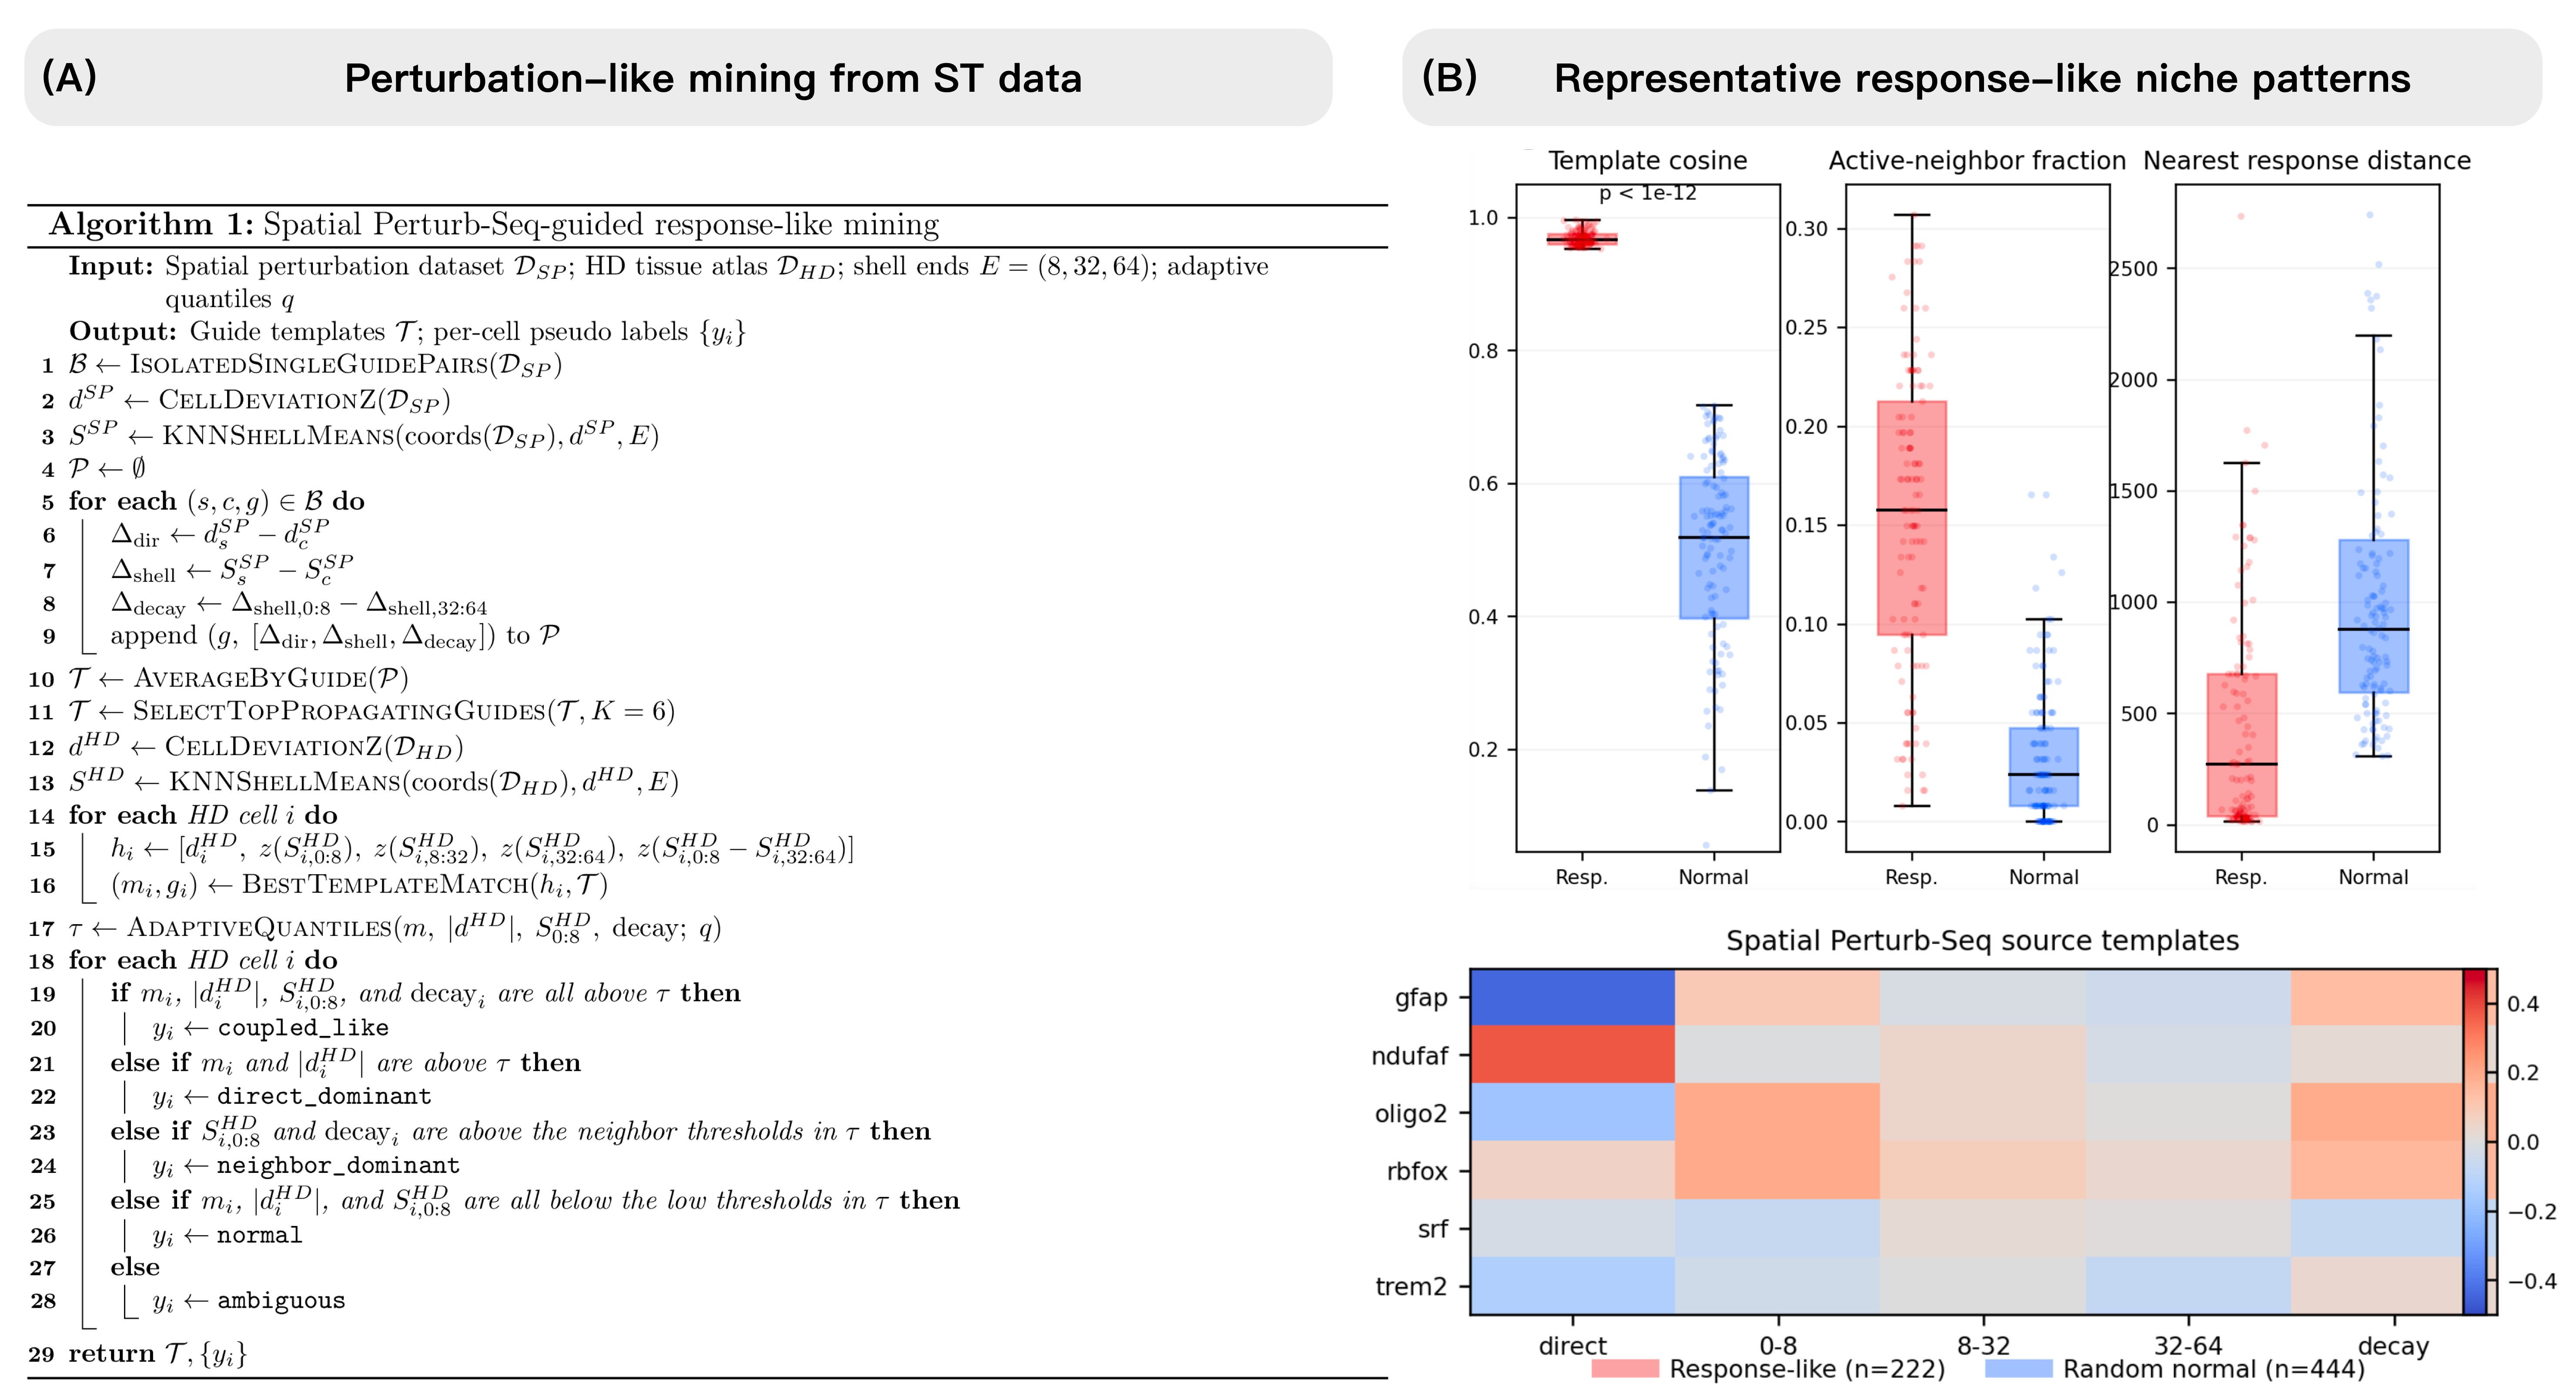
\includegraphics[width=0.82\linewidth]{TURB1.png}

\vspace{0.4em}

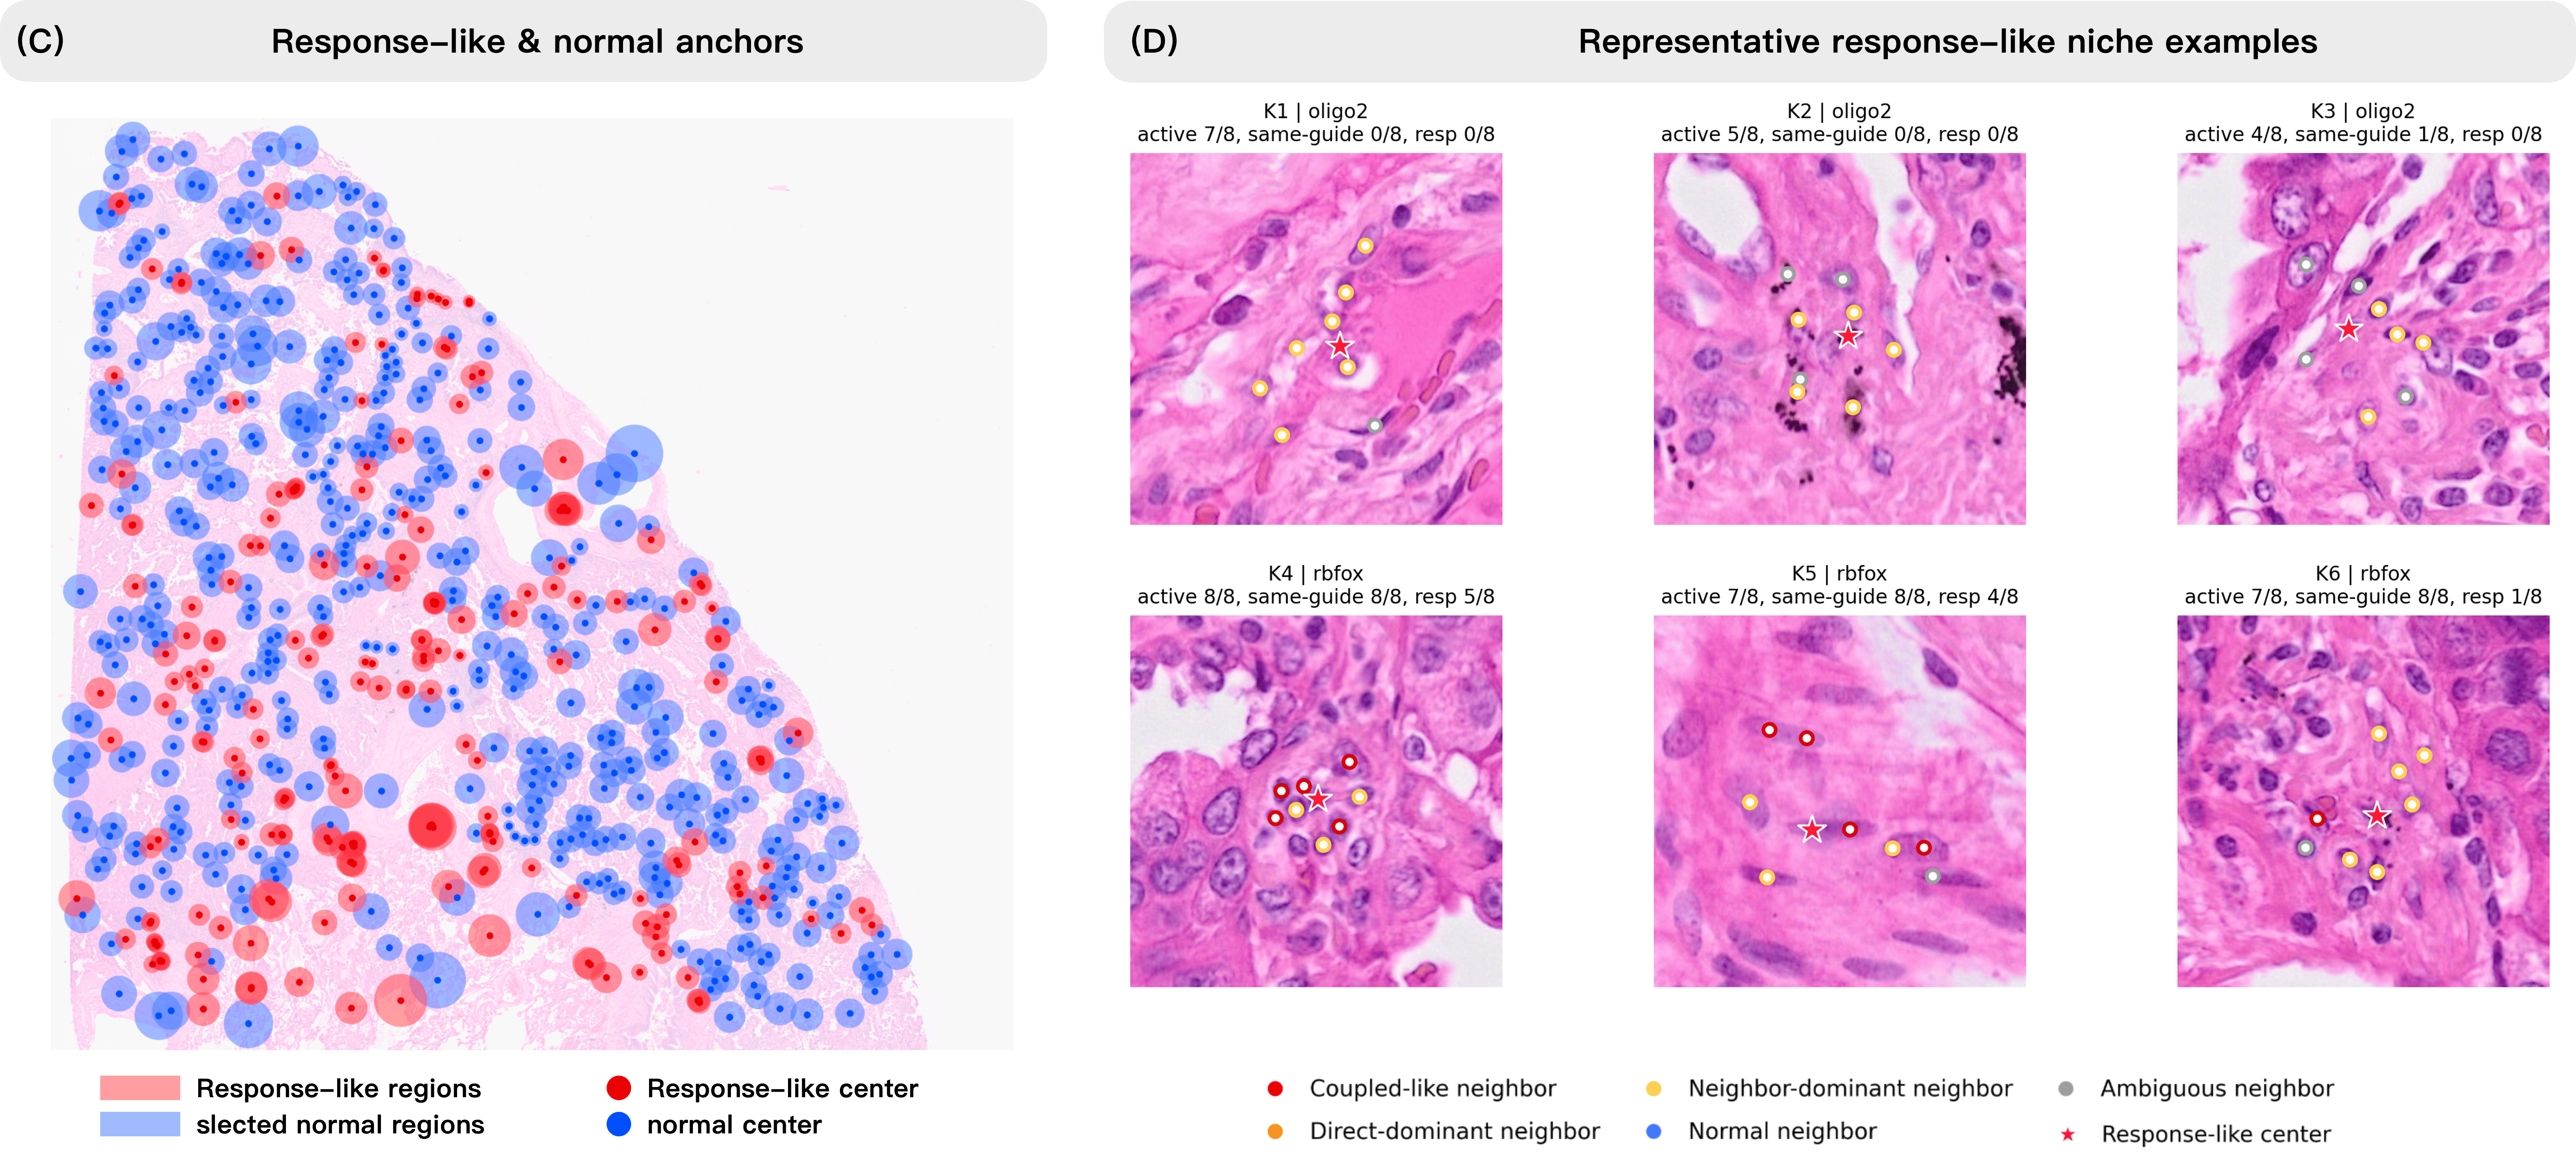
\includegraphics[width=0.82\linewidth]{TURB2.png}
\caption{Mining communication-rich microenvironments from unperturbed reference ST. Candidate tissue regions are scored for spatially local cell--cell structure, including neighborhood geometry, cell-state organization, and communication compatibility. Selected communication-rich and background regions pretrain a frozen reference microenvironment encoder without perturbation labels.}
\label{fig:app_st_mining}
\end{figure}

\subsection{Communication-rich microenvironment mining}
\label{app:communication_microenvironment_mining}

\paragraph{Mining communication-rich microenvironments from unperturbed reference ST.}
The second data component uses unperturbed high-resolution spatial transcriptomics to identify reference microenvironments with strong local communication structure. These data are not used as perturbation labels. Instead, they provide spatial contexts in which cell--cell communication is plausible.

For each organ or tissue source, we construct a reference ST corpus
\[
\mathcal B=\{R_1,\ldots,R_N\},
\]
where each region $R$ contains local cells or spatial bins with expression profiles, coordinates, and inferred or annotated cell states. Within each region, we define a local cell--cell graph
\[
E_R=\{(i,j):\|s_i-s_j\|_2\le r,\ i\neq j\},
\]
where $r$ is a spatial interaction radius. A candidate communication program may correspond to a ligand--receptor pair, a ligand--target module, or a learned gene program. For a candidate gene pair or communication program $(p,q)$, the local communication score is
\[
C_R(p,q)
=
\frac{1}{|E_R|}
\sum_{(i,j)\in E_R}
\tilde x_{ip}\tilde x_{jq}
\exp\left(
-\frac{\|s_i-s_j\|_2^2}{2\sigma_d^2}
\right),
\]
where $\tilde x_{ip}$ and $\tilde x_{jq}$ are normalized expression values for the signal-side and response-side genes. This score favors regions where a signal-side program and a response-side program are jointly active in spatially adjacent cells.

Each region is summarized by its strongest communication programs and local tissue context:
\[
h_R=[\bar z_R,\pi_R,\mathrm{TopK}\{C_R(p,q)\},\rho_R],
\]
where $\bar z_R$ is the mean expression embedding, $\pi_R$ is the cell-type composition, and $\rho_R$ summarizes local spatial density and neighborhood geometry. Regions are selected as high-communication microenvironments if their communication scores exceed a reference-ST quantile threshold and both signal-side and response-side populations are sufficiently represented:
\[
\mathcal R_{\mathrm{high}}
=
\left\{
R\in\mathcal B:
\max_{(p,q)}C_R(p,q)\ge Q_{1-\eta},
\ n_{\mathrm{signal}}(R)\ge n_{\min},
\ n_{\mathrm{response}}(R)\ge n_{\min}
\right\}.
\]
We also retain low-communication regions as background controls. Together, these regions form a reference library of communication-rich and communication-poor tissue contexts.

The mined regions are used to pretrain the reference microenvironment encoder. They expose the model to diverse local gene-coupling and cell--cell communication patterns, but do not define perturbation-response targets. During perturbation training, Spatial Perturb-Seq patches supervise the signed response field, while the frozen microenvironment encoder supplies niche context for ring-aware propagation refinement.

The corresponding reference communication prior is
\[
A_{\mathrm{CCC}}(i,j)
=
\sum_{(p,q)\in\mathcal G}
\beta_{pq}
\tilde x_{ip}\tilde x_{jq}
\exp\left(
-\frac{\|s_i-s_j\|_2^2}{2\sigma_d^2}
\right),
\]
where $\mathcal G$ is the set of communication programs and $\beta_{pq}$ is a program weight learned from the mined regions. This prior acts as a gate for plausible communication paths. It does not define the perturbation target; effective propagated responses are still learned from true spatial perturbation supervision.

\subsection{Mouse perturbation-like microenvironment mining from HD and Xenium reference ST}
\label{app:mouse_microenvironment_mining}

To expand the reference microenvironment corpus beyond the single true spatial perturbation benchmark, we mined perturbation-like local regions from unperturbed mouse-brain HD and Xenium spatial transcriptomics datasets. These regions are not treated as perturbation-response labels. Instead, they provide diverse mouse-brain microenvironments in which specific gene programs are locally enriched and can be paired with matched background regions for reference-prior pretraining.

We used seven perturbation-like program templates:
\texttt{interferon\_inflammatory\_like},
\texttt{trem2\_microglia\_dam\_like},
\texttt{astrocyte\_gliosis\_like},
\texttt{oligodendrocyte\_myelin\_like},
\texttt{neuronal\_activity\_srf\_like},
\texttt{rbfox\_neuronal\_like}, and
\texttt{mitochondrial\_oxidative\_like}.
Across two HD mouse-brain sections and three Xenium mouse-brain studies, this procedure screened 392,962 cells, identified 1,619 perturbation-like positive anchors, and generated 9,316 anchor--normal local pairs. The mined anchors cover inflammatory/IFN-like, TREM2 microglia/DAM-like, astrocyte gliosis-like, oligodendrocyte/myelin-like, neuronal activity/SRF-like, Rbfox neuronal/RNA-splicing-like, and mitochondrial/OXPHOS-like microenvironments.

These mined anchor--normal pairs are used to pretrain the reference microenvironment encoder. The encoder learns local niche structure, program co-activation, and cell--cell plausibility from unperturbed reference ST. During supervised spatial perturbation training, however, the signed response targets still come only from Spatial Perturb-seq PPP pairs. Thus, the mined HD/Xenium regions mitigate the limited diversity of available ground-truth spatial perturbation data without converting unperturbed ST into pseudo perturbation labels.

\begin{figure}[t]
\centering
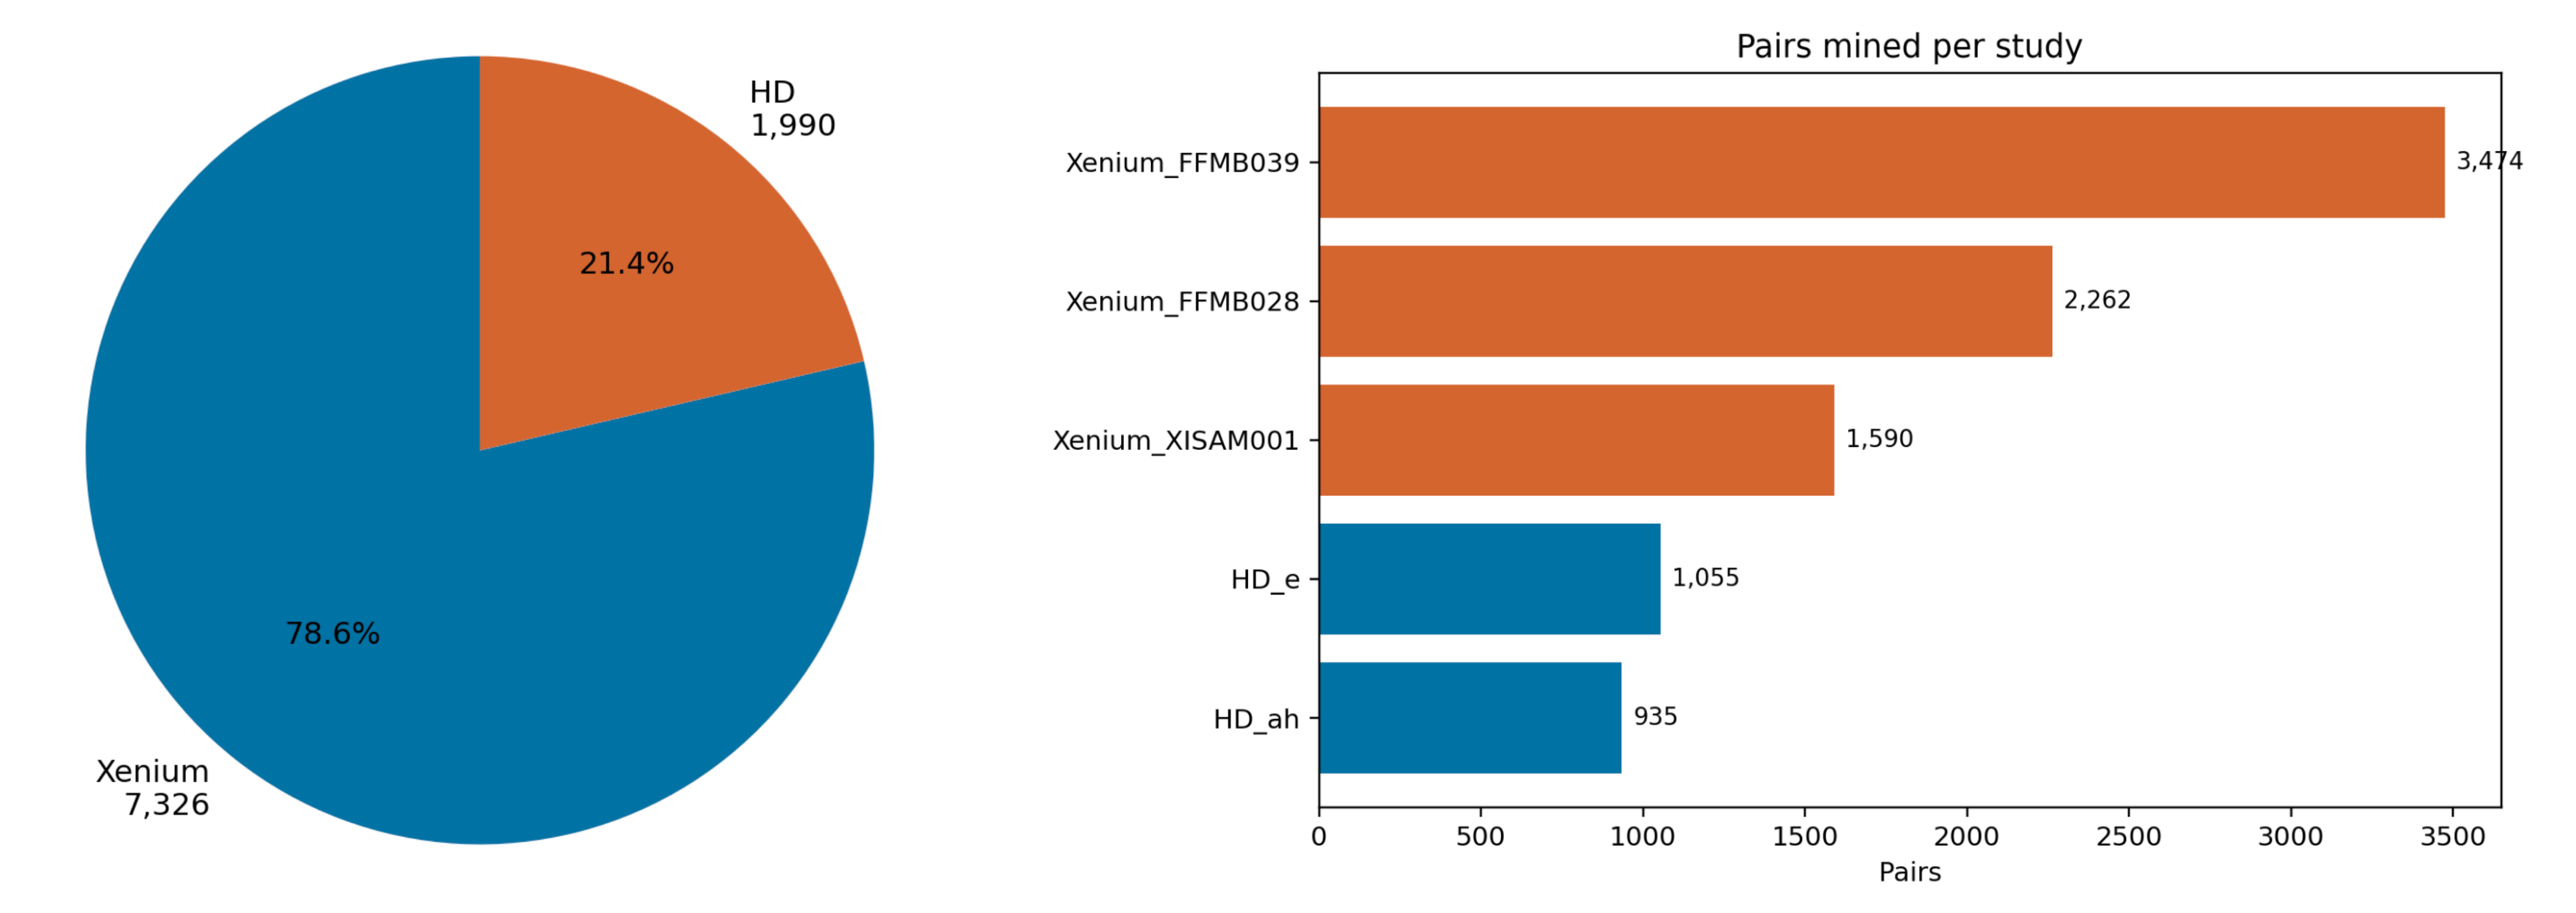
\includegraphics[width=\linewidth]{mouse_mining.png}
\vspace{-0.6em}
\caption{Mouse-brain perturbation-like microenvironment mining from HD and Xenium reference ST. Program-enriched local regions are identified from unperturbed mouse-brain spatial transcriptomics and paired with matched background regions. These mined pairs pretrain the frozen microenvironment prior used by \methodname{}, but do not define perturbation-response targets.}
\label{fig:mouse_mining}
\vspace{-0.6em}
\end{figure}

\begin{table*}[t]
\centering
\caption{Study-level mouse-brain perturbation-like microenvironment mining results. Positive anchors denote local regions assigned to one perturbation-like program. Pairs denote mined anchor--normal local pairs used for reference microenvironment prior pretraining.}
\label{tab:mouse_mining_studies}
\scriptsize
\setlength{\tabcolsep}{3pt}
\renewcommand{\arraystretch}{1.10}
\begin{tabularx}{\textwidth}{@{}llrrr>{\raggedright\arraybackslash}X@{}}
\toprule
Study & Modality & Cells & Anchors & Pairs & Inferred perturbation-like areas \\
\midrule

\texttt{HD\_e} &
HD &
51,190 &
211 &
1,055 &
Rbfox-like neuronal/RNA-splicing response (114); mitochondrial/OXPHOS stress-like response (95); oligodendrocyte/myelin lineage-like response (2). \\

\texttt{HD\_ah} &
HD &
54,298 &
187 &
935 &
Rbfox-like neuronal/RNA-splicing response (124); mitochondrial/OXPHOS stress-like response (53); oligodendrocyte/myelin lineage-like response (10). \\

\texttt{Xenium\_FFMB039} &
Xenium &
162,033 &
579 &
3,474 &
Oligodendrocyte/myelin-like response (575); neuronal activity/SRF-like response (4). \\

\texttt{Xenium\_FFMB028} &
Xenium &
63,173 &
377 &
2,262 &
Interferon/inflammatory-like response (286); TREM2 microglia/DAM-like response (84); astrocyte gliosis-like response (7). \\

\texttt{Xenium\_XISAM001} &
Xenium &
62,268 &
265 &
1,590 &
Neuronal activity/SRF-like response (166); interferon/inflammatory-like response (80); TREM2 microglia/DAM-like response (19). \\

\midrule
Total &
-- &
392,962 &
1,619 &
9,316 &
587 oligodendrocyte/myelin-like; 366 interferon/inflammatory-like; 238 Rbfox neuronal/RNA-splicing-like; 170 neuronal activity/SRF-like; 148 mitochondrial/OXPHOS-like; 103 TREM2 microglia/DAM-like; 7 astrocyte gliosis-like anchors. \\

\bottomrule
\end{tabularx}
\end{table*}

\subsection{Comparison to available spatial and single-cell perturbation resources}
\label{app:resource_comparison}

\begin{table*}[t]
\centering
\caption{Comparison to available spatial and single-cell perturbation resources. ``Ready for propagation'' means that the public data can directly define cell-resolved direct-effect-to-neighbor propagation targets with perturbation assignment, transcriptome-scale expression, and spatial coordinates measured in the same cells.}
\label{tab:app_resource_comparison}
\footnotesize
\setlength{\tabcolsep}{2.5pt}
\renewcommand{\arraystretch}{1.18}
\begin{tabular}{@{}p{0.18\linewidth}ccccccp{0.34\linewidth}@{}}
\toprule
Resource / assay &
\makecell[c]{Single\\cell} &
\makecell[c]{Spatial\\coords} &
\makecell[c]{Pert.\\barcode} &
\makecell[c]{Whole\\transcriptome} &
\makecell[c]{Native\\tissue} &
\makecell[c]{Ready for\\propagation} &
Reason not used as an external benchmark \\
\midrule
Spatial Perturb-Seq &
Yes & Yes & Yes & Yes & Yes & Yes &
Primary benchmark in this work; it jointly provides cell-level perturbation assignment, transcriptome-scale expression, and spatial coordinates in intact mouse brain. \\

Dissociated Perturb-Seq / single-cell perturbation collections &
Yes & No & Yes & Yes & No & No &
Useful for direct-effect prediction, but dissociation removes spatial neighborhoods and native neighbor context. \\

Unperturbed spatial transcriptomics atlases &
Partial & Yes & No & Partial & Yes & No &
Provide reference tissue context and coordinates, but no perturbation assignment or perturbation-response labels. \\

Perturb-map / Pro-Code spatial CRISPR screens &
Partial & Yes & Yes & Partial & Yes & No &
Perturbation identity is spatially mapped through protein or imaging barcodes, but the public readouts do not provide matched whole-transcriptome cell-level response fields for this neighbor-propagation benchmark. \\

Perturb-FISH and related imaging-barcode spatial screens &
Yes & Yes & Yes & Targeted & Yes & No &
Combine spatial imaging transcriptomics with guide detection, but current public readouts are not benchmark-ready paired whole-transcriptome neighbor-response fields. \\

Emerging spatial CRISPR co-sequencing platforms &
Partial & Yes & Yes & Partial / Yes & Yes & Not yet &
Promising platforms can co-measure spatial transcriptomes and guide RNAs, but are not yet available as public, benchmark-ready, cell-resolved paired response-field datasets for this task. \\

Multi-condition spatial transcriptomics studies &
Partial & Yes & Condition & Partial & Yes & No &
Compare perturbed or disease conditions across samples or slices, but do not provide cell-level perturbation barcodes identifying direct-effect cells and neighbor propagation targets. \\
\bottomrule
\end{tabular}
\end{table*}

\subsection{Full method equations and training details}
\label{app:method_full_details}

\paragraph{Graph notation.}
Each local perturbation sample is a graph $P=(V,E)$ with $m=64$ cells. Cell $i$ has matched-control expression $x_i\in\mathbb R^G$, coarse cell state $c_i$, relative coordinate $p_i$, direct-effect-relative geometry $g_i$, direct-effect indicator $a_i\in\{0,1\}$, and direct-effect profile $d_i\in\mathbb R^G$. The direct-effect profile is nonzero only on direct-effect cells. Directed edge $(i,j)$ has features $e_{ij}$, including relative geometry, cell-type-pair indicators, and communication-compatibility score $q_{ij}$. The model predicts $\widehat\Delta_i\in\mathbb R^G$ and reconstructs $\widehat x_i^{\mathrm{post}}=x_i+\widehat\Delta_i$.

\paragraph{Niche-impact residualization.}
The response decomposition is
\[
\Delta_i=I_i^{\mathrm{niche}}+I_i^{\mathrm{prop}} .
\]
The niche module removes perturbation information:
\[
\widehat I_i^{\mathrm{niche}}
=
f_{\mathrm{niche}}(x,c,p,e;\ a=0,d=0).
\]
The propagation target is
\[
I_i^{\mathrm{prop},\star}
=
\Delta_i-\widehat I_i^{\mathrm{niche}} .
\]
Thus, matched-control variation, local tissue composition, and geometry are absorbed by $\widehat I_i^{\mathrm{niche}}$, while directed propagation learns perturbation-conditioned propagation impact.

\paragraph{Direct-effect and neighbor initialization.}
Each cell embedding is
\[
h_i=\phi_x(x_i)+\phi_c(c_i)+\phi_p(p_i)+\phi_g(g_i).
\]
Neighbor and direct-effect states are initialized separately:
\[
n_i^0=\phi_N(h_i),
\qquad
u_i^0=a_i\phi_D([h_i,d_i,g_i]).
\]
This construction prevents neighbor cells from directly seeing the perturbation input.

\paragraph{Directed direct-effect-to-neighbor propagation.}
For propagation layer $\ell$, a direct-effect-to-neighbor message from direct-effect cell $i$ to neighbor cell $j$ is
\[
g_{ij}^{\ell}
=
\sigma\!\left(
\phi_a([u_i^\ell,n_j^\ell,e_{ij}])
+
w_{\mathrm{comm}}q_{ij}
\right),
\]
\[
\mu_{ij}^{\ell}
=
g_{ij}^{\ell}
\phi_\mu([u_i^\ell,n_j^\ell,e_{ij}]).
\]
Neighbor messages are aggregated over direct-effect cells:
\[
\bar\mu_j^\ell
=
\sum_{i:a_i=1}\mu_{ij}^{\ell},
\qquad
n_j^{\ell+1}
=
\phi_u([n_j^\ell,\bar\mu_j^\ell]).
\]
After $L$ layers, the base propagation module predicts
\[
\widehat I_i^{\mathrm{prop},\mathrm{base}}
=
a_i\psi_{\mathrm{direct}}(u_i^L)
+
(1-a_i)\psi_{\mathrm{neighbor}}(n_i^L).
\]

\paragraph{Reference-ST niche encoder.}
The reference encoder is pretrained on unperturbed ST regions and then frozen. It returns cell-level niche embeddings, a patch-level niche token, and edge-plausibility estimates:
\[
\{z_i^{\mathrm{ref}}\},\ n_P^{\mathrm{ref}},\ b_{ij}^{\mathrm{ref}},\ u_{ij}^{\mathrm{ref}}
=
f_{\mathrm{ref}}(x,c,p,e).
\]
The neighbor-side niche summary is
\[
o_P=
\left[
n_P^{\mathrm{ref}},
\frac{1}{|V_N|}
\sum_{j\in V_N}z_j^{\mathrm{ref}}
\right],
\]
where $V_N$ is the neighbor set. The frozen reference context is injected through zero-initialized adapters:
\[
u_i^0
\leftarrow
u_i^0
+
a_i\lambda_D\phi_D^{\mathrm{ref}}(o_P),
\qquad
n_i^0
\leftarrow
n_i^0
+
(1-a_i)\lambda_N\phi_N^{\mathrm{ref}}(o_P).
\]
Because $\lambda_D$ and $\lambda_N$ are initialized at zero, the reference-ST module begins as the base propagation model and learns only microenvironment corrections.

\paragraph{Ring-aware response feedback.}
The ST-conditioned module first predicts $\widehat I_i^{\mathrm{prop},(1)}$. Neighbor response strength is scored by
\[
\kappa_j
=
\frac{1}{G}
\sum_{g=1}^{G}
\left|
\widehat I_{jg}^{\mathrm{prop},(1)}
\right|.
\]
The top 5\% neighbor cells by $\kappa_j$ are selected as feedback cells $F$. Neighbors are partitioned by direct-effect-relative distance into three rings: nearest eight neighbors, next 24 neighbors, and remaining neighbors. For each ring $b$, the model constructs a response token:
\[
t_b
=
\phi_b
\left(
\left[
\mathrm{mean}_{j\in F\cap B_b}\widehat I_j^{\mathrm{prop},(1)},
\mathrm{std}_{j\in F\cap B_b}\widehat I_j^{\mathrm{prop},(1)}
\right]
\right).
\]
The direct-effect cells receive the average ring token, and each neighbor receives the token for its ring. A second directed propagation pass produces $\widehat I_i^{\mathrm{prop},(2)}$.

\paragraph{Restricted ring-aware correction.}
The final ST-conditioned propagation impact is
\[
\widehat I_i^{\mathrm{prop},\mathrm{st}}
=
\widehat I_i^{\mathrm{prop},(1)}
+
\lambda_i
\mathbf 1[i\in V_D\cup F]
\left(
\widehat I_i^{\mathrm{prop},(2)}-\widehat I_i^{\mathrm{prop},(1)}
\right),
\]
where $V_D$ is the direct-effect set, $F$ is the feedback-neighbor set, and neighbor-side $\lambda_i$ is ring-specific. This restriction lets high-response regions feed back into the model without allowing the second pass to uniformly rewrite all neighbor cells.

\paragraph{Final response prediction.}
The final prediction is
\[
\widehat\Delta_i
=
\widehat I_i^{\mathrm{niche}}
+
(1-\alpha)\widehat I_i^{\mathrm{prop},\mathrm{base}}
+
\alpha\widehat I_i^{\mathrm{prop},\mathrm{st}},
\]
with $\alpha=0.65$ selected on validation data. This is a propagation-delta blend. The reconstructed post-state expression is
\[
\widehat x_i^{\mathrm{post}}
=
x_i+\widehat\Delta_i.
\]

\paragraph{Reference-ST pretraining objective.}
The reference microenvironment encoder is trained without perturbation labels:
\[
\mathcal L_{\mathrm{ref}}
=
2.0\mathcal L_{\mathrm{masked\text{-}program}}
+
1.0\mathcal L_{\mathrm{neighborhood}}
+
0.25\mathcal L_{\mathrm{patch\text{-}hist}}
+
0.25\mathcal L_{\mathrm{edge}}.
\]
The terms supervise masked gene-program reconstruction, neighborhood-conditioned program prediction, patch cell-type composition, and pseudo edge-plausibility prediction. These objectives teach local niche structure and communication plausibility, but not perturbation response.

\paragraph{Propagation-impact objective.}
After niche-impact residualization, the propagation module is trained with neighbor-focused supervision:
\[
\mathcal L_{\mathrm{prop}}
=
1.0\mathcal L_{\mathrm{neighbor}}
+
0.3\mathcal L_{\mathrm{ring}}
+
0.3\mathcal L_{\mathrm{post}}
+
0.1\mathcal L_{\mathrm{rank}}.
\]
$\mathcal L_{\mathrm{neighbor}}$ is a Huber loss on high-confidence neighbor-cell propagation impacts. $\mathcal L_{\mathrm{ring}}$ supervises ring-aggregated response after adding the niche-impact baseline. $\mathcal L_{\mathrm{post}}$ supervises reconstructed post-state expression $x_i+\widehat I_i^{\mathrm{niche}}+\widehat I_i^{\mathrm{prop}}$. $\mathcal L_{\mathrm{rank}}$ is a pairwise ranking loss over per-patch gene-response magnitudes. The direct-effect-cell loss weight is set to zero in the strongest propagation setting so that the easier direct-effect signal does not dominate neighbor propagation.

\subsection{Full gene-centric neighbor-response validation}
\label{app:full_gene_centric_validation}


\subsection{Strict grouped guide-out stability}
\label{sec:guide_stratified_stability}

To test perturbation-level generalization, we use a strict grouped guide-out split. The perturbation guides \textit{fasn}, \textit{stk39}, and \textit{trem2} are jointly excluded from training and validation, yielding 992 unseen-guide graphs. With observed sender-side direct-effect seeds, \methodname{} reaches pooled neighbor/ring Pearson $0.596/0.451$, outperforming elastic-net patch-summary regression $(0.334/0.142)$ and a Generic Graph Transformer without CCC priors $(0.497/0.395)$. Per-guide performance remains stable across all three held-out perturbations, indicating that the grouped guide-out result is not driven by a single guide.

\begin{table*}[t]
\centering
\footnotesize
\setlength{\tabcolsep}{4pt}
\renewcommand{\arraystretch}{1.04}
\caption{\textbf{Strict grouped guide-out evaluation.}
The perturbation guides \textit{fasn}, \textit{stk39}, and \textit{trem2} are held out jointly during training and validation. The table reports per-guide performance for \methodname{} under observed and zero direct-effect seeds, together with exact-task baseline performance on the same unseen-guide graphs. Neighbor, centered, and ring scores are Pearson correlations.}
\label{tab:strict_grouped_guide_out}
\resizebox{\linewidth}{!}{%
\begin{tabular}{llrcccc}
\toprule
\textbf{Model} &
\textbf{Held-out guide} &
\textbf{$n$ graphs} &
\textbf{Input} &
\textbf{Neighbor} &
\textbf{Centered} &
\textbf{Ring} \\
\midrule

\rowcolor{gray!12}
\multicolumn{7}{l}{\textit{\methodname{} on the strict grouped guide-out split.}} \\

\methodname{} &
\textit{fasn} &
413 &
Observed seed &
0.5982 &
\textemdash &
0.4540 \\

\methodname{} &
\textit{stk39} &
351 &
Observed seed &
0.5978 &
\textemdash &
0.4573 \\

\methodname{} &
\textit{trem2} &
228 &
Observed seed &
0.6006 &
\textemdash &
0.4562 \\

\methodname{} &
Overall &
992 &
Observed seed &
0.5964 &
\textemdash &
0.4514 \\

\addlinespace[1pt]
\methodname{} &
\textit{fasn} &
413 &
Zero seed &
0.5983 &
\textemdash &
0.4449 \\

\methodname{} &
\textit{stk39} &
351 &
Zero seed &
0.5979 &
\textemdash &
0.4466 \\

\methodname{} &
\textit{trem2} &
228 &
Zero seed &
0.6013 &
\textemdash &
0.4517 \\

\methodname{} &
Overall &
992 &
Zero seed &
0.5964 &
\textemdash &
0.4374 \\

\midrule
\rowcolor{gray!12}
\multicolumn{7}{l}{\textit{Exact-task baselines on the same unseen-guide graphs.}} \\

Elastic-net patch-summary &
\textit{fasn} &
413 &
Patch summary &
0.3345 &
0.4820 &
0.1376 \\

Elastic-net patch-summary &
\textit{stk39} &
351 &
Patch summary &
0.3352 &
0.4838 &
0.1366 \\

Elastic-net patch-summary &
\textit{trem2} &
228 &
Patch summary &
0.3398 &
0.4856 &
0.1393 \\

Generic Graph Transformer, no CCC &
\textit{fasn} &
413 &
Graph only &
0.4991 &
0.5121 &
0.3918 \\

Generic Graph Transformer, no CCC &
\textit{stk39} &
351 &
Graph only &
0.4984 &
0.5120 &
0.3956 \\

Generic Graph Transformer, no CCC &
\textit{trem2} &
228 &
Graph only &
0.5009 &
0.5148 &
0.3887 \\

\bottomrule
\end{tabular}
}
\end{table*}

The \methodname{} rows are consistent across the three unseen perturbations: observed-seed neighbor Pearson stays between $0.5978$ and $0.6006$, and observed-seed ring Pearson stays between $0.4540$ and $0.4573$. Zero-seed evaluation preserves nearly identical neighbor Pearson but reduces ring Pearson to $0.4449$--$0.4517$. The two baseline families remain substantially lower in ring Pearson across all three guides, supporting strict grouped guide-out generalization rather than a single-guide artifact.

\subsection{Guide-stratified stability on the held-out Spatial Perturb-Seq test set}
\label{app:guide_stratified_stability}

To test whether the held-out Spatial Perturb-Seq result is dominated by a small
number of perturbation guides, we stratified the frozen \methodname{} predictions
by guide identity on the held-out test split. This is a guide-stratified stability
audit of the same held-out test predictions, not a leave-one-guide-out retraining
experiment. We include guides with at least 20 held-out test patches.

Across 14 guides, performance is stable and closely matches the overall test result.
The overall held-out split reaches neighbor/ring Pearson $0.6842/0.4574$ over
928 patches. The mean across guide strata is $0.6851 \pm 0.0044$ for neighbor
Pearson and $0.4604 \pm 0.0203$ for ring Pearson. Per-guide neighbor Pearson ranges
from $0.6767$ to $0.6952$, and per-guide ring Pearson ranges from $0.4276$ to
$0.4956$. This indicates that the aggregate held-out performance is not driven by
a single guide or a small subset of guides.

\begin{figure*}[t]
    \centering
    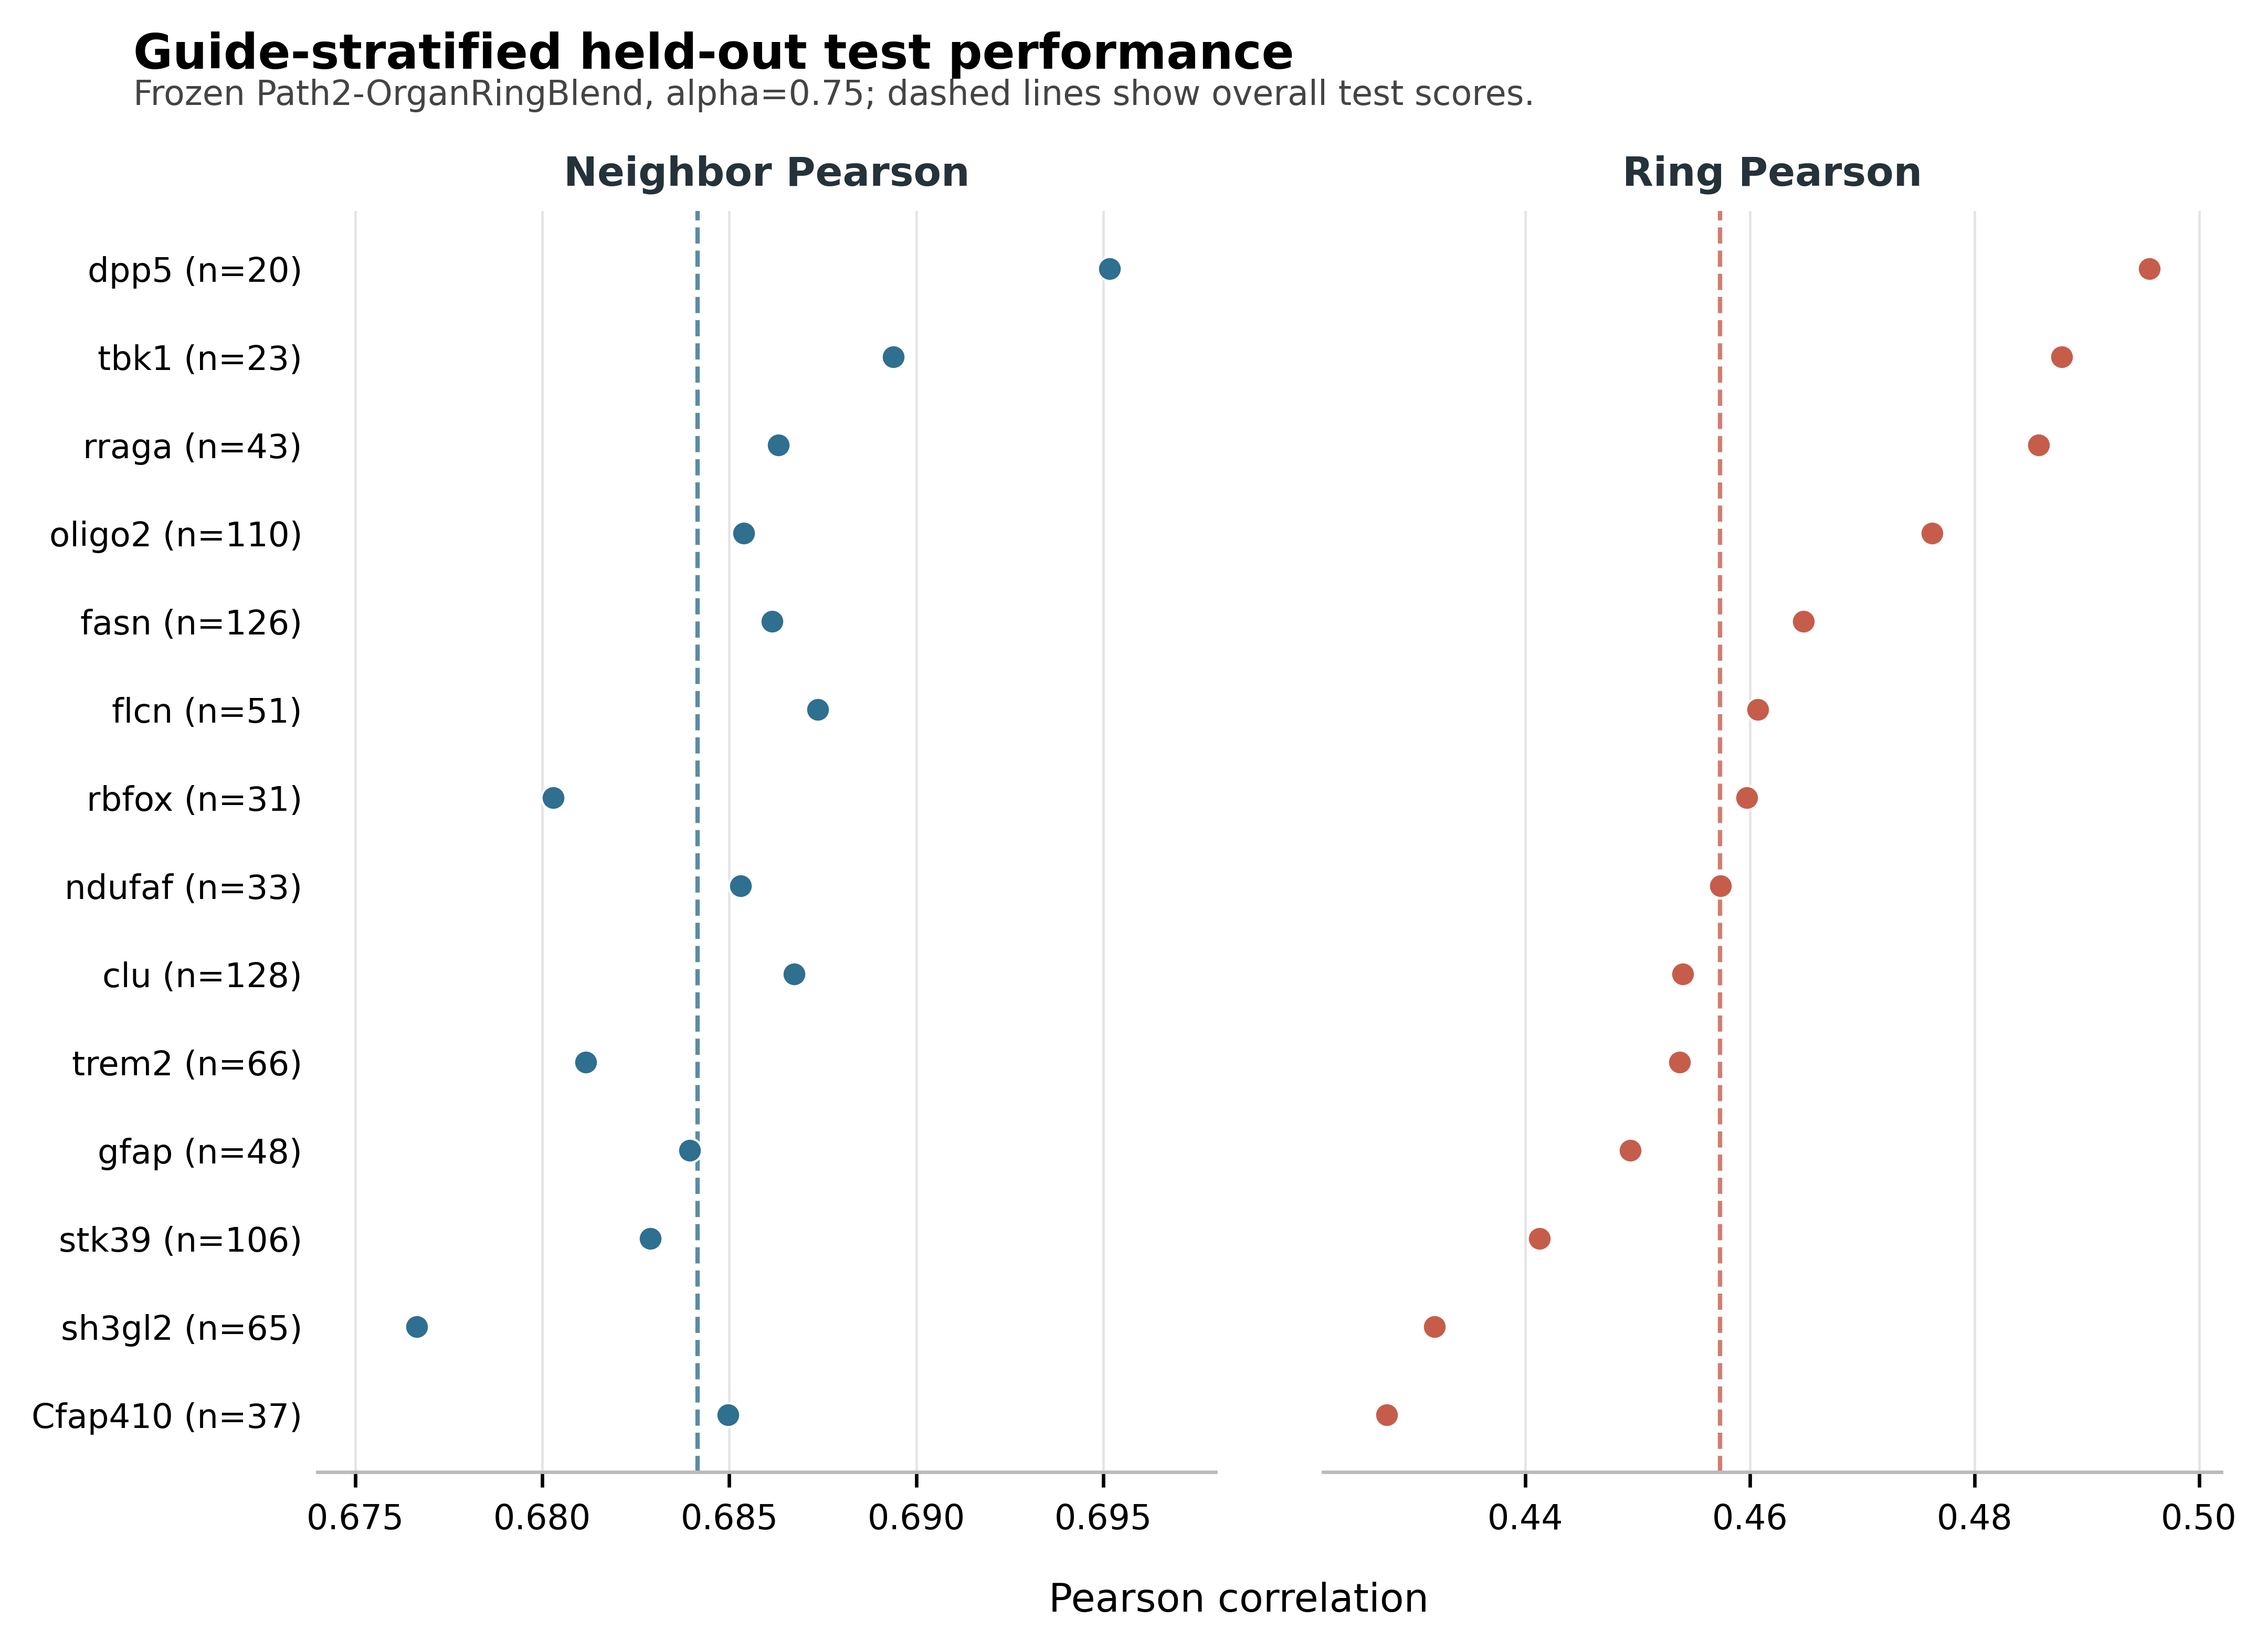
\includegraphics[width=0.8\textwidth]{path2_organringblend_guide_stratified_heldout_test_dotplot.png}
    \caption{\textbf{Guide-stratified held-out test stability.}
    Frozen \methodname{} predictions are stratified by guide identity on the same
    held-out Spatial Perturb-Seq test split. Dashed vertical lines show the overall
    held-out test scores. Across 14 guides with at least 20 test patches, both
    neighbor and ring Pearson remain close to the overall result, indicating that
    the benchmark performance is not driven by a small number of guides.}
    \label{fig:guide_stratified_stability}
\end{figure*}

\begin{table}[t]
\centering
\footnotesize
\setlength{\tabcolsep}{5pt}
\renewcommand{\arraystretch}{1.06}
\caption{\textbf{Guide-stratified held-out test performance.}
The first two rows summarize the overall test split and the mean across guide strata.
Per-guide rows include guides with at least 20 held-out test patches.}
\label{tab:guide_stratified_stability}
\begin{tabular}{lccc}
\toprule
\textbf{Readout} & \textbf{Test patches} & \textbf{Neighbor Pearson} & \textbf{Ring Pearson} \\
\midrule
Overall test split & 928 & 0.6842 & 0.4574 \\
Mean across guides & 887 & $0.6851 \pm 0.0044$ & $0.4604 \pm 0.0203$ \\
\midrule
\textit{clu} & 128 & 0.6867 & 0.4540 \\
\textit{fasn} & 126 & 0.6861 & 0.4648 \\
\textit{oligo2} & 110 & 0.6854 & 0.4762 \\
\textit{stk39} & 106 & 0.6829 & 0.4413 \\
\textit{trem2} & 66 & 0.6812 & 0.4537 \\
\textit{sh3gl2} & 65 & 0.6767 & 0.4319 \\
\textit{flcn} & 51 & 0.6874 & 0.4607 \\
\textit{gfap} & 48 & 0.6839 & 0.4493 \\
\textit{rraga} & 43 & 0.6863 & 0.4857 \\
\textit{Cfap410} & 37 & 0.6850 & 0.4276 \\
\textit{ndufaf} & 33 & 0.6853 & 0.4574 \\
\textit{rbfox} & 31 & 0.6803 & 0.4597 \\
\textit{tbk1} & 23 & 0.6894 & 0.4878 \\
\textit{dpp5} & 20 & 0.6952 & 0.4956 \\
\bottomrule
\end{tabular}
\end{table}

% If not already defined:
% \newcommand{\pmv}[2]{#1\,{\scriptsize$\pm$}\,#2}

\begin{figure*}[t]
\centering
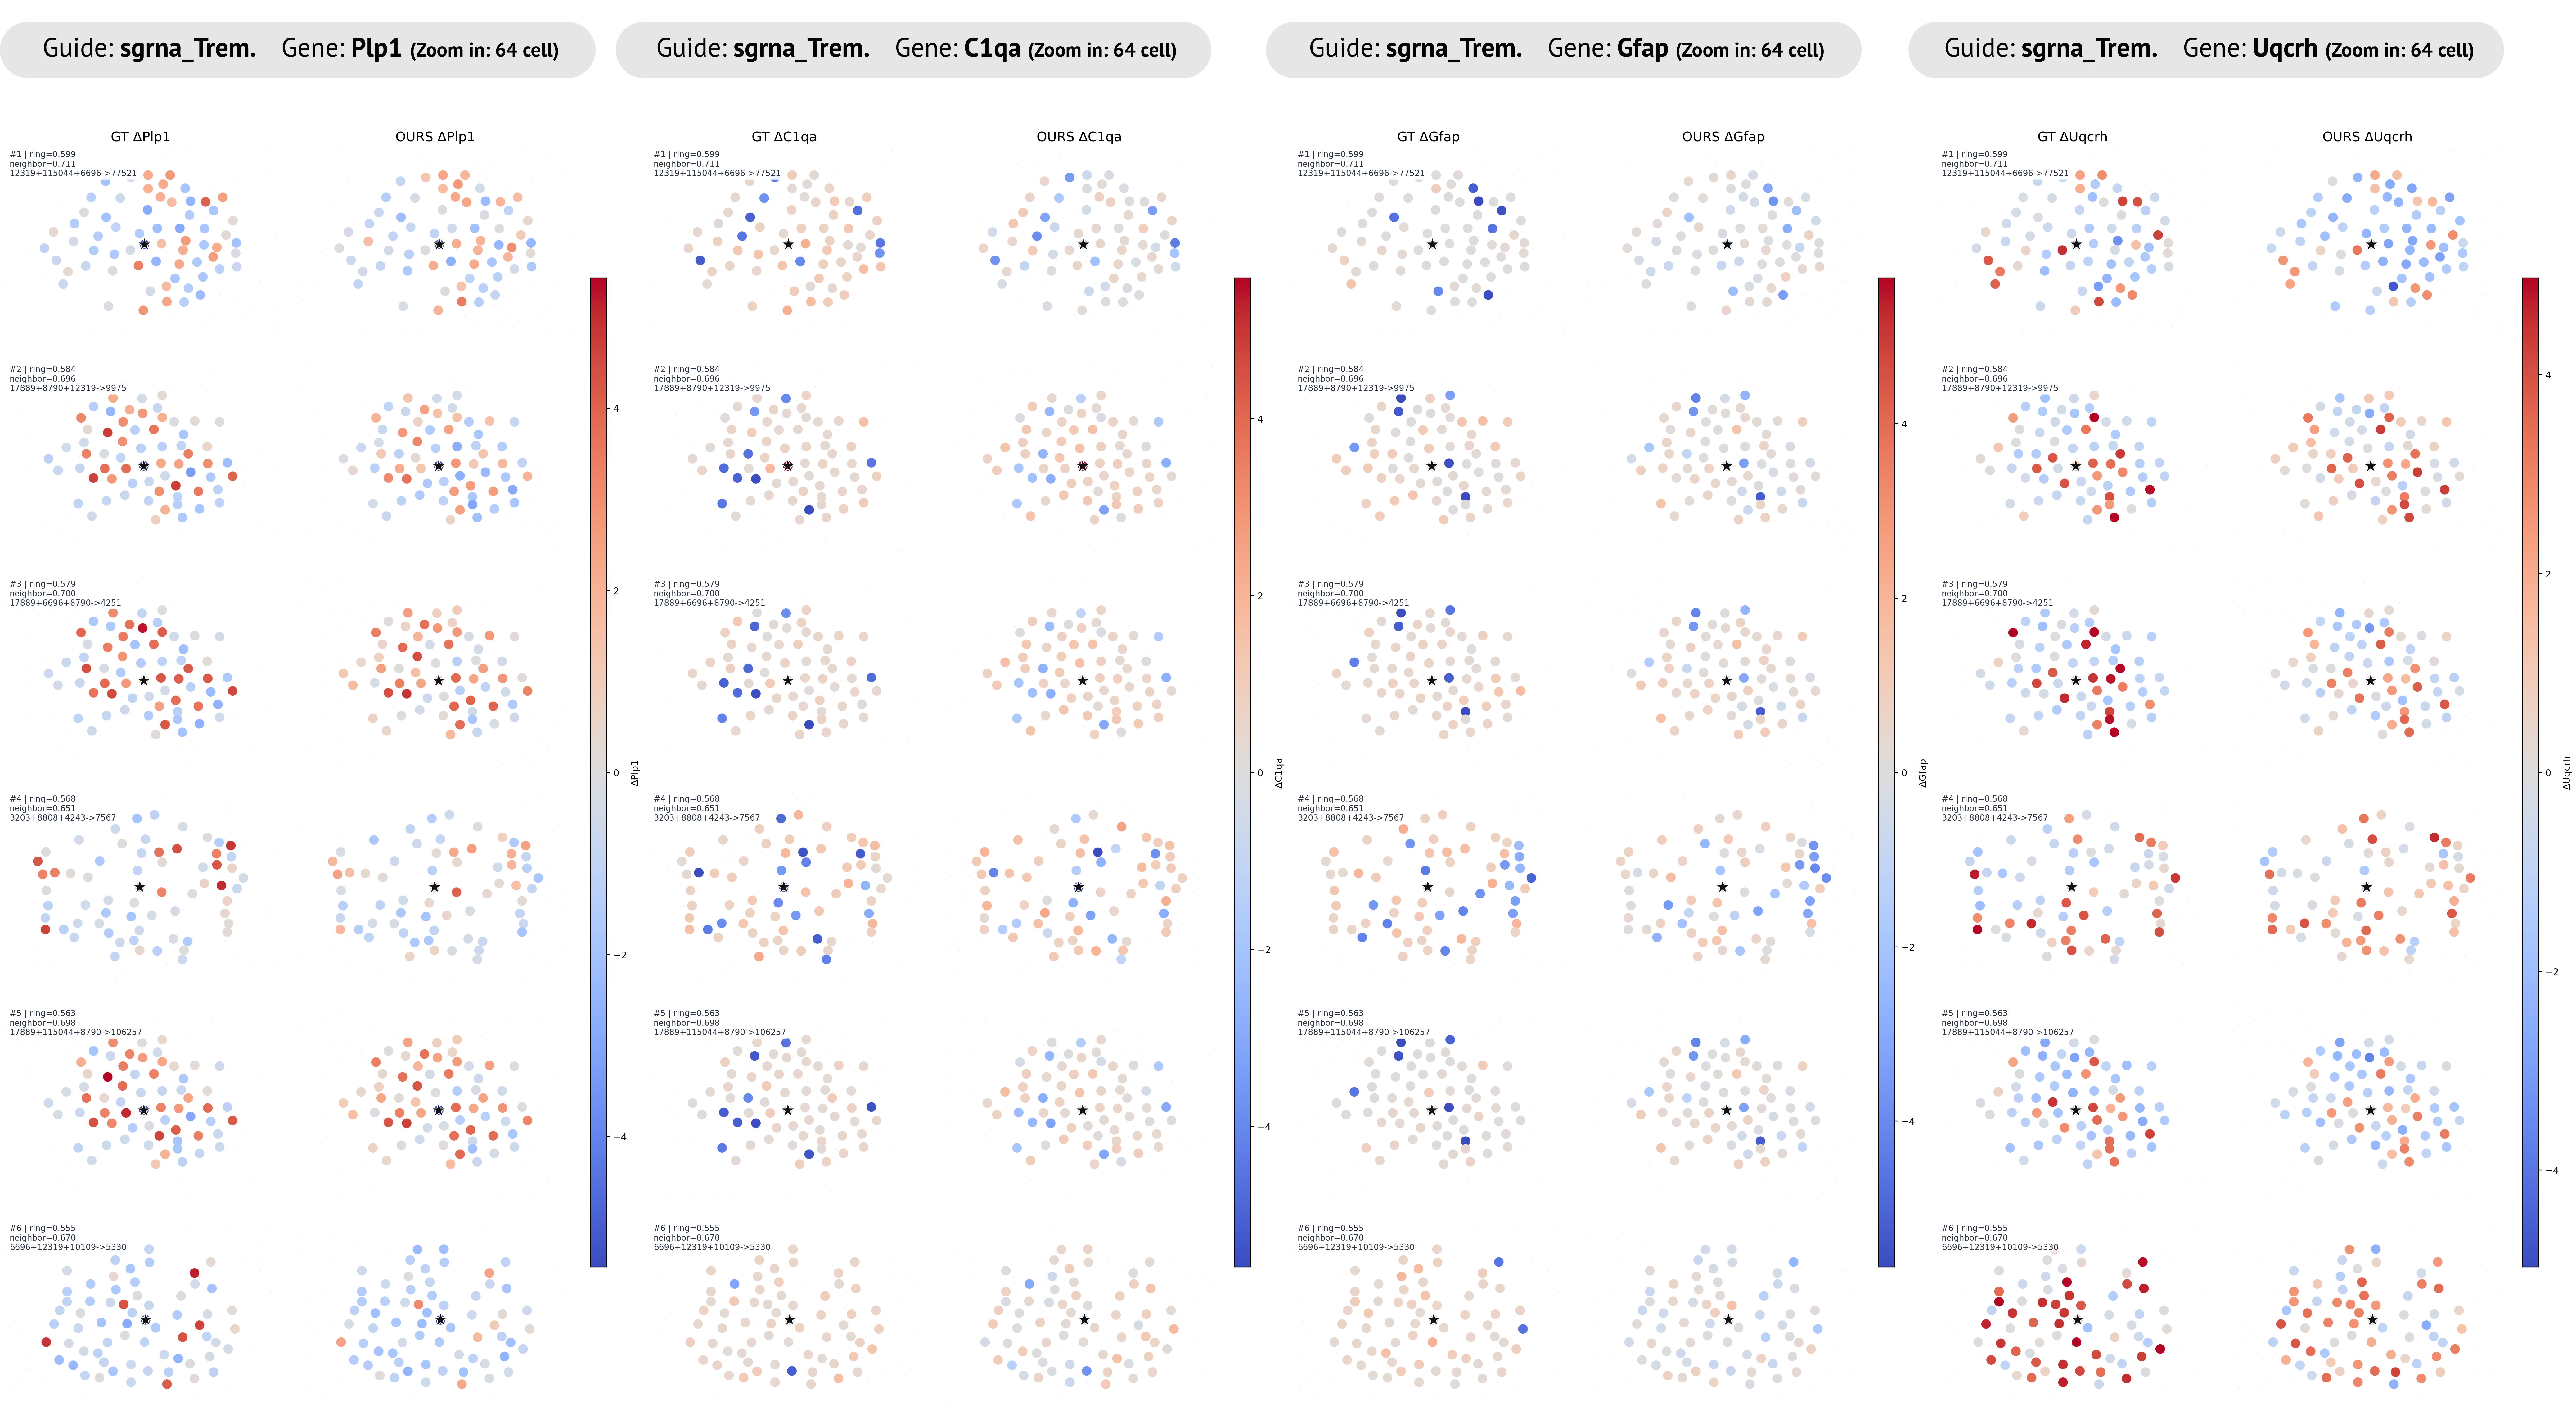
\includegraphics[width=0.98\linewidth]{main_result.png}
\caption{\textbf{Expanded real-data validation results on the Spatial Perturb-Seq mouse-brain benchmark.}
This appendix figure provides the full-resolution version of the main real-data evaluation summarized in \Cref{fig:main_exp}, including spatial response maps, local neighbor-cell neighborhoods, and gene-level recovery patterns under the block-held-out matched-control setting.}
\label{fig:app_main_result}
\end{figure*}

\begin{table*}[t]
\centering
\footnotesize
\setlength{\tabcolsep}{3.2pt}
\renewcommand{\arraystretch}{1.02}
\caption{\textbf{Full gene-centric neighbor-cell performance on the Spatial Perturb-Seq benchmark.}
Values are computed over neighbor cells and reported as estimate with uncertainty.
Gray rows mark perturbation-related, high-variance, and high-change gene groups.}
\label{tab:app_validation_summary}
\resizebox{\linewidth}{!}{%
\begin{tabular}{@{}lcccccccc@{}}
\toprule
\textbf{Gene} &
\textbf{Mean $|\Delta|$} &
\textbf{Pearson} &
\textbf{Spearman} &
\textbf{Cosine} &
\textbf{$R^2$} &
\textbf{MAE} &
\textbf{RMSE} &
\textbf{Sign acc.} \\
\midrule

\rowcolor{gray!18}
\multicolumn{9}{@{}l}{\textbf{\textit{Perturbation-related genes.}}} \\
\textit{Gfap}   & \pmv{0.966}{0.016} & \pmv{0.788}{0.005} & \pmv{0.313}{0.013} & \pmv{0.788}{0.005} & \pmv{0.621}{0.007} & \pmv{0.785}{0.008} & \pmv{1.047}{0.011} & \pmv{0.716}{0.007} \\
\textit{Trem2}  & \pmv{0.324}{0.006} & \pmv{0.266}{0.005} & \pmv{0.053}{0.012} & \pmv{0.243}{0.005} & \pmv{0.047}{0.004} & \pmv{0.449}{0.005} & \pmv{0.968}{0.010} & \pmv{0.586}{0.009} \\
\textit{C1qa}   & \pmv{0.996}{0.012} & \pmv{0.835}{0.003} & \pmv{0.309}{0.009} & \pmv{0.835}{0.003} & \pmv{0.694}{0.005} & \pmv{0.690}{0.005} & \pmv{0.916}{0.007} & \pmv{0.788}{0.004} \\
\textit{Olig2}  & \pmv{0.287}{0.007} & \pmv{0.184}{0.006} & \pmv{-0.004}{0.012} & \pmv{0.180}{0.004} & \pmv{0.018}{0.004} & \pmv{0.385}{0.005} & \pmv{0.865}{0.011} & \pmv{0.546}{0.010} \\
\textit{Opalin} & \pmv{0.868}{0.014} & \pmv{0.781}{0.003} & \pmv{0.383}{0.012} & \pmv{0.775}{0.003} & \pmv{0.601}{0.006} & \pmv{0.722}{0.006} & \pmv{0.991}{0.008} & \pmv{0.652}{0.007} \\

\midrule
\rowcolor{gray!18}
\multicolumn{9}{@{}l}{\textbf{\textit{Top five high-variance genes.}}} \\
\textit{Ptgds}  & \pmv{1.984}{0.010} & \pmv{0.805}{0.004} & \pmv{0.810}{0.004} & \pmv{0.805}{0.004} & \pmv{0.645}{0.007} & \pmv{1.087}{0.011} & \pmv{1.382}{0.014} & \pmv{0.913}{0.003} \\
\textit{Plp1}   & \pmv{1.743}{0.014} & \pmv{0.737}{0.005} & \pmv{0.745}{0.006} & \pmv{0.737}{0.005} & \pmv{0.533}{0.009} & \pmv{1.174}{0.013} & \pmv{1.501}{0.016} & \pmv{0.807}{0.004} \\
\textit{Ywhaz}  & \pmv{2.020}{0.010} & \pmv{0.772}{0.005} & \pmv{0.776}{0.005} & \pmv{0.759}{0.005} & \pmv{0.540}{0.011} & \pmv{1.274}{0.017} & \pmv{1.588}{0.019} & \pmv{0.898}{0.003} \\
\textit{Uqcrh}  & \pmv{1.971}{0.010} & \pmv{0.790}{0.004} & \pmv{0.773}{0.005} & \pmv{0.788}{0.004} & \pmv{0.616}{0.008} & \pmv{1.123}{0.012} & \pmv{1.416}{0.015} & \pmv{0.894}{0.003} \\
\textit{Sst}    & \pmv{2.031}{0.014} & \pmv{0.773}{0.006} & \pmv{0.733}{0.007} & \pmv{0.770}{0.006} & \pmv{0.580}{0.011} & \pmv{1.245}{0.019} & \pmv{1.581}{0.024} & \pmv{0.862}{0.006} \\

\midrule
\rowcolor{gray!18}
\multicolumn{9}{@{}l}{\textbf{\textit{High-change genes.}}} \\
\textit{Cycs}   & \pmv{2.356}{0.015} & \pmv{0.851}{0.003} & \pmv{0.693}{0.007} & \pmv{0.843}{0.004} & \pmv{0.708}{0.007} & \pmv{1.161}{0.014} & \pmv{1.462}{0.018} & \pmv{0.923}{0.003} \\
\textit{Nme2}   & \pmv{2.347}{0.014} & \pmv{0.874}{0.002} & \pmv{0.714}{0.005} & \pmv{0.873}{0.002} & \pmv{0.762}{0.004} & \pmv{1.051}{0.010} & \pmv{1.328}{0.012} & \pmv{0.951}{0.002} \\
\textit{Rack1}  & \pmv{2.333}{0.011} & \pmv{0.880}{0.002} & \pmv{0.678}{0.006} & \pmv{0.872}{0.003} & \pmv{0.759}{0.005} & \pmv{1.056}{0.011} & \pmv{1.332}{0.014} & \pmv{0.928}{0.003} \\
\textit{Ptma}   & \pmv{2.203}{0.012} & \pmv{0.882}{0.002} & \pmv{0.678}{0.005} & \pmv{0.878}{0.002} & \pmv{0.769}{0.004} & \pmv{1.008}{0.010} & \pmv{1.265}{0.012} & \pmv{0.966}{0.002} \\
\textit{Psmb4}  & \pmv{2.197}{0.008} & \pmv{0.826}{0.004} & \pmv{0.810}{0.004} & \pmv{0.826}{0.004} & \pmv{0.673}{0.007} & \pmv{1.132}{0.013} & \pmv{1.421}{0.015} & \pmv{0.926}{0.003} \\

\bottomrule
\end{tabular}
}
\end{table*}

% =========================================================
% Appendix: Controlled synthetic LR-propagation benchmark
% Required packages:
% \usepackage{booktabs}
% \usepackage{graphicx}
% \usepackage{subcaption}
% \usepackage{array}
% =========================================================

\subsection{Controlled synthetic LR-propagation validation}
\label{app:synthetic_lr_validation}

To complement the exact cell-resolved Spatial Perturb-Seq benchmark, we constructed
a controlled synthetic LR-propagation benchmark using external in vivo mouse
Perturb-seq direct-effect signatures from Jin \textit{et al.} (GSE157977), unperturbed
mouse-brain spatial graphs, and a NicheNet/LR-based neighbor-response simulator.
This setting is not biological ground truth; it is a controlled validation benchmark
for testing whether direct-effect-conditioned neighbor propagation is learnable when the
response field is generated under known communication rules.

The main synthetic split contains 432 graphs, with 252/72/108 train/validation/test
graphs. Random, clustered, and interface direct-effect geometries are balanced across
splits, as are perturbation strengths $0.75$, $1.25$, and $2.0$. We report
Neighbor Pearson and ring-level Pearson as the primary readouts. Niche-module-only
predictions are near zero, indicating that the synthetic target is not explained by
tissue context alone. Synthetic fine-tuning recovers the held-out response field,
whereas direct transfer from the real-data pretrained model remains weak, consistent
with simulator-distribution mismatch.

\begin{figure*}[t]
    \centering
    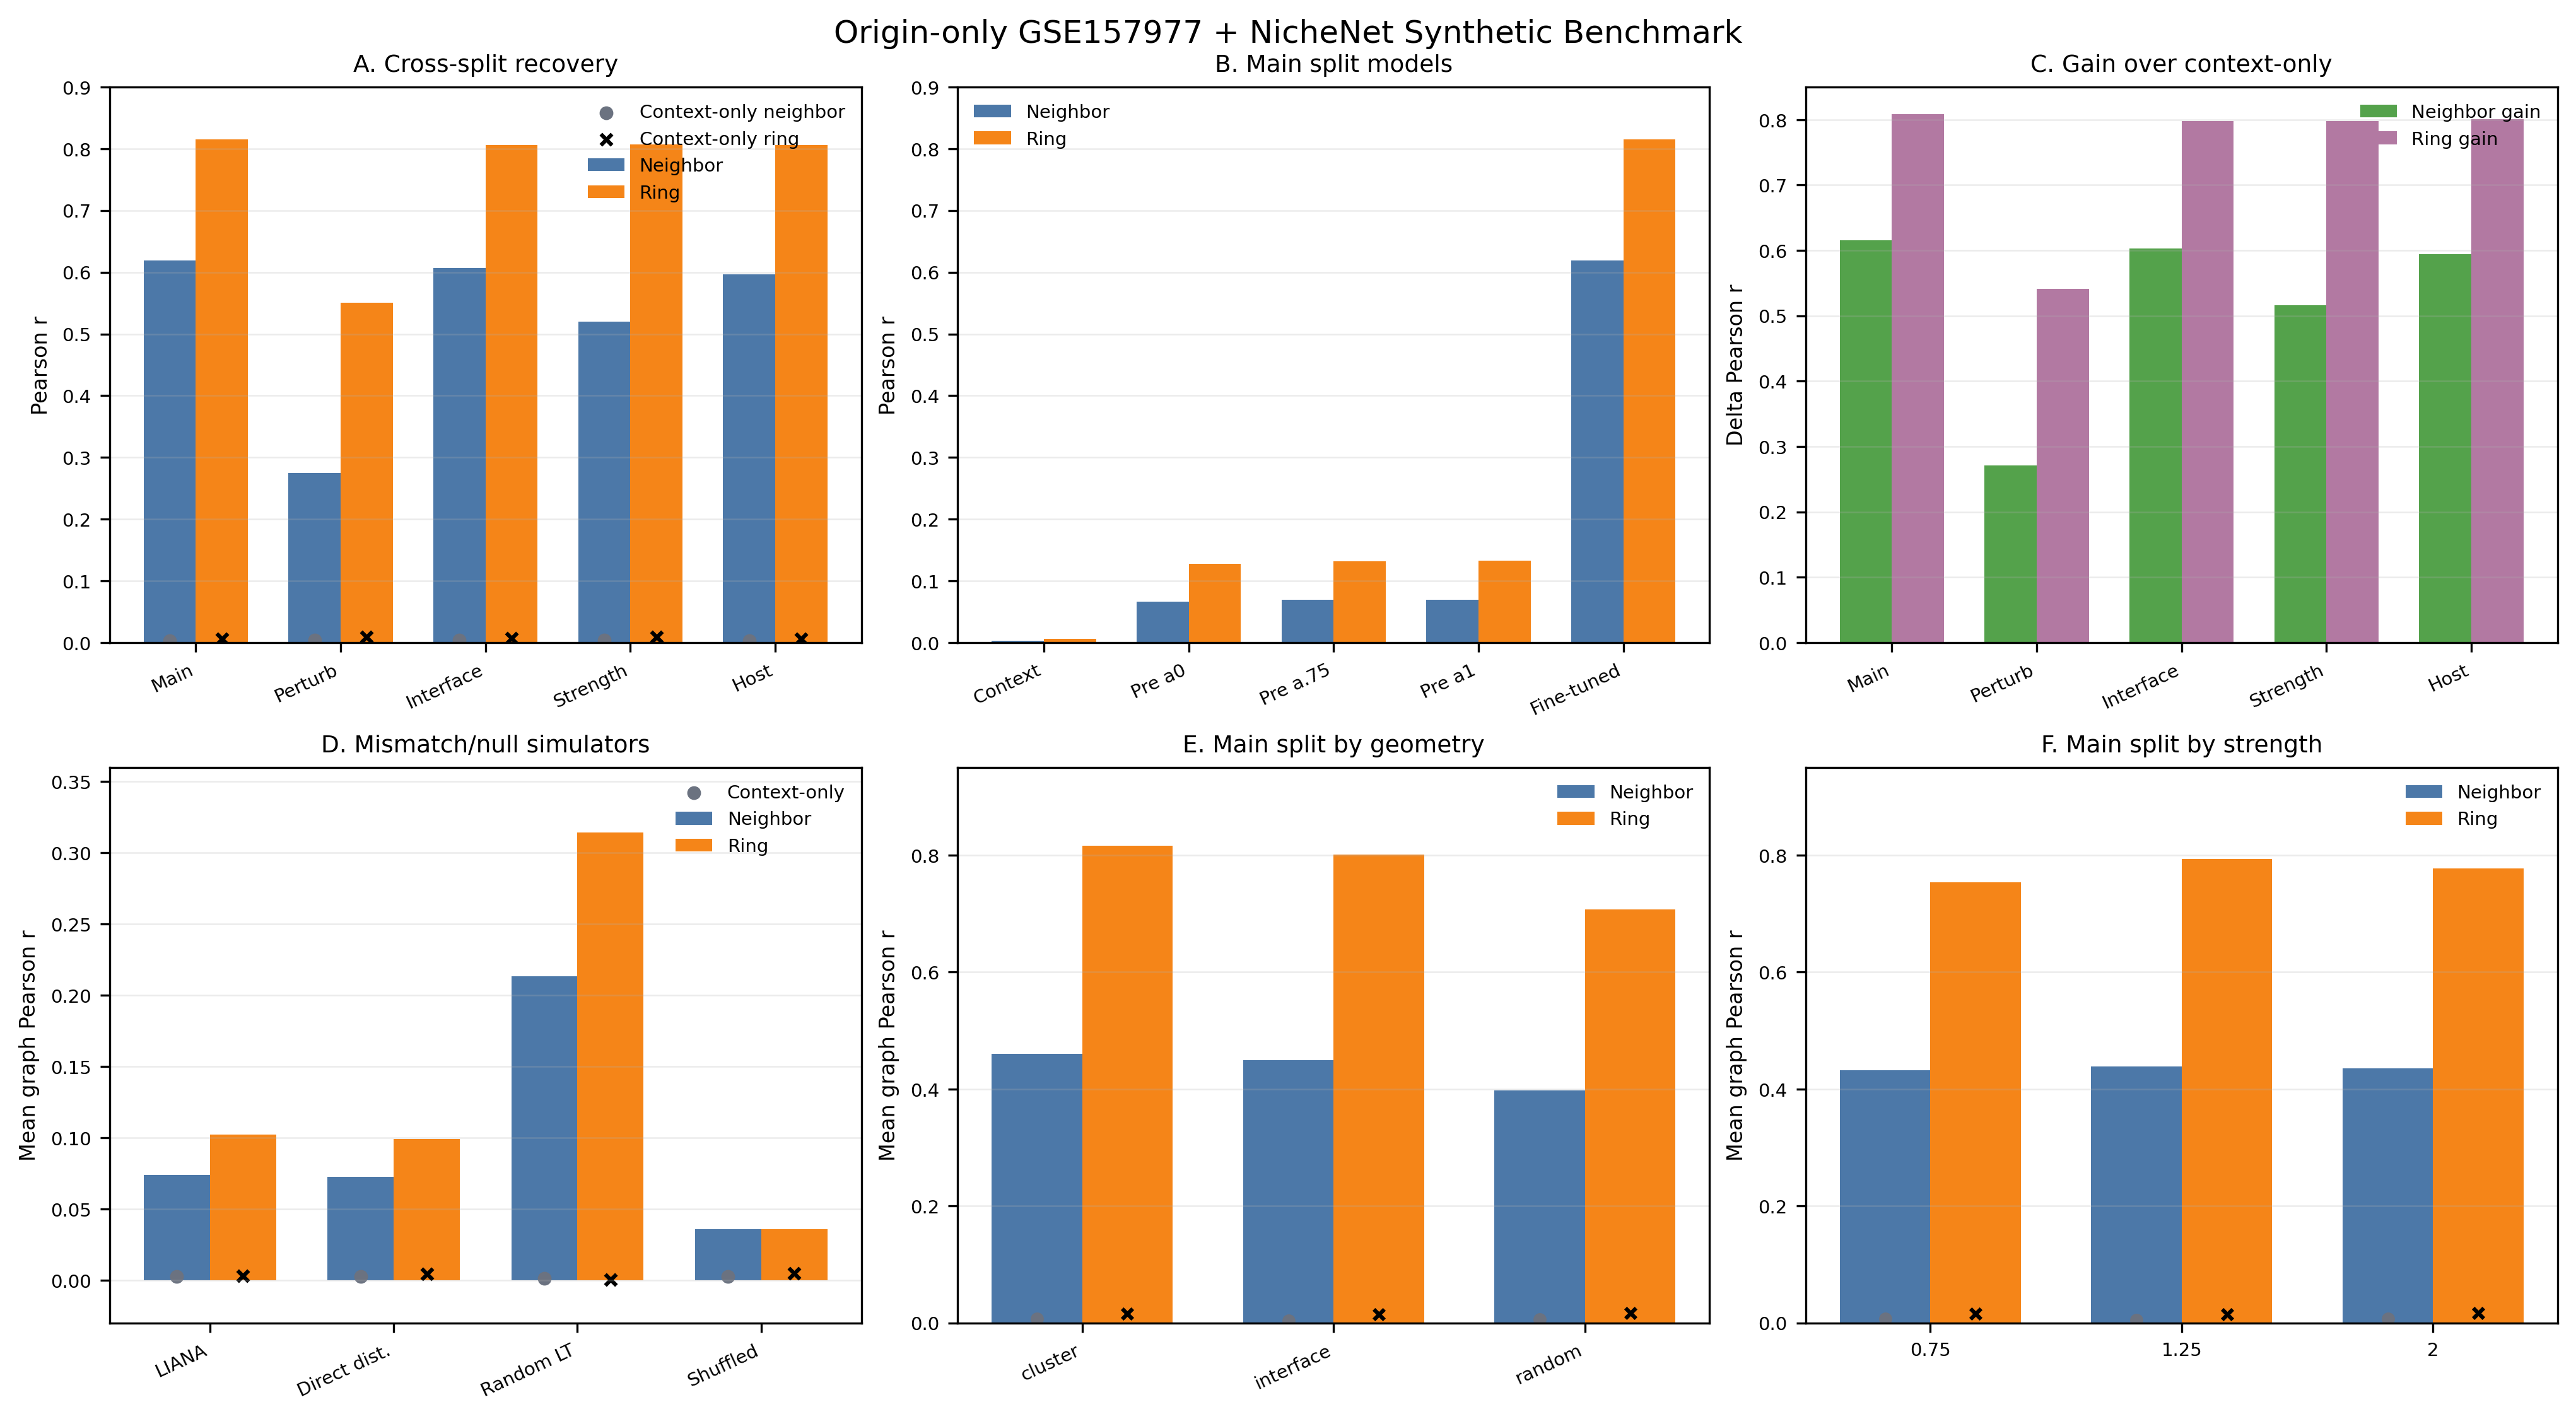
\includegraphics[width=\textwidth]{synthetic_lr_summary.png}
    \caption{\textbf{Controlled synthetic LR-propagation validation.}
    (A) Cross-split recovery across the main stratified split and held-out perturbation,
    interface geometry, strength, and host-patch splits. Niche-module-only predictions remain
    near zero, while synthetic-trained models recover neighbor and ring-level
    structure. (B) Main-split model comparison. Direct transfer from the real-data
    pretrained model is weak, whereas synthetic fine-tuning recovers the synthetic
    target. (C) Gain over the niche-module-only baseline across cross-split settings.
    (D) Simulator mismatch and null-control settings. (E) Main-split performance by
    geometry strategy. (F) Main-split performance by perturbation strength.}
    \label{fig:synthetic_lr_summary}
\end{figure*}

\begin{figure}[t]
    \centering
    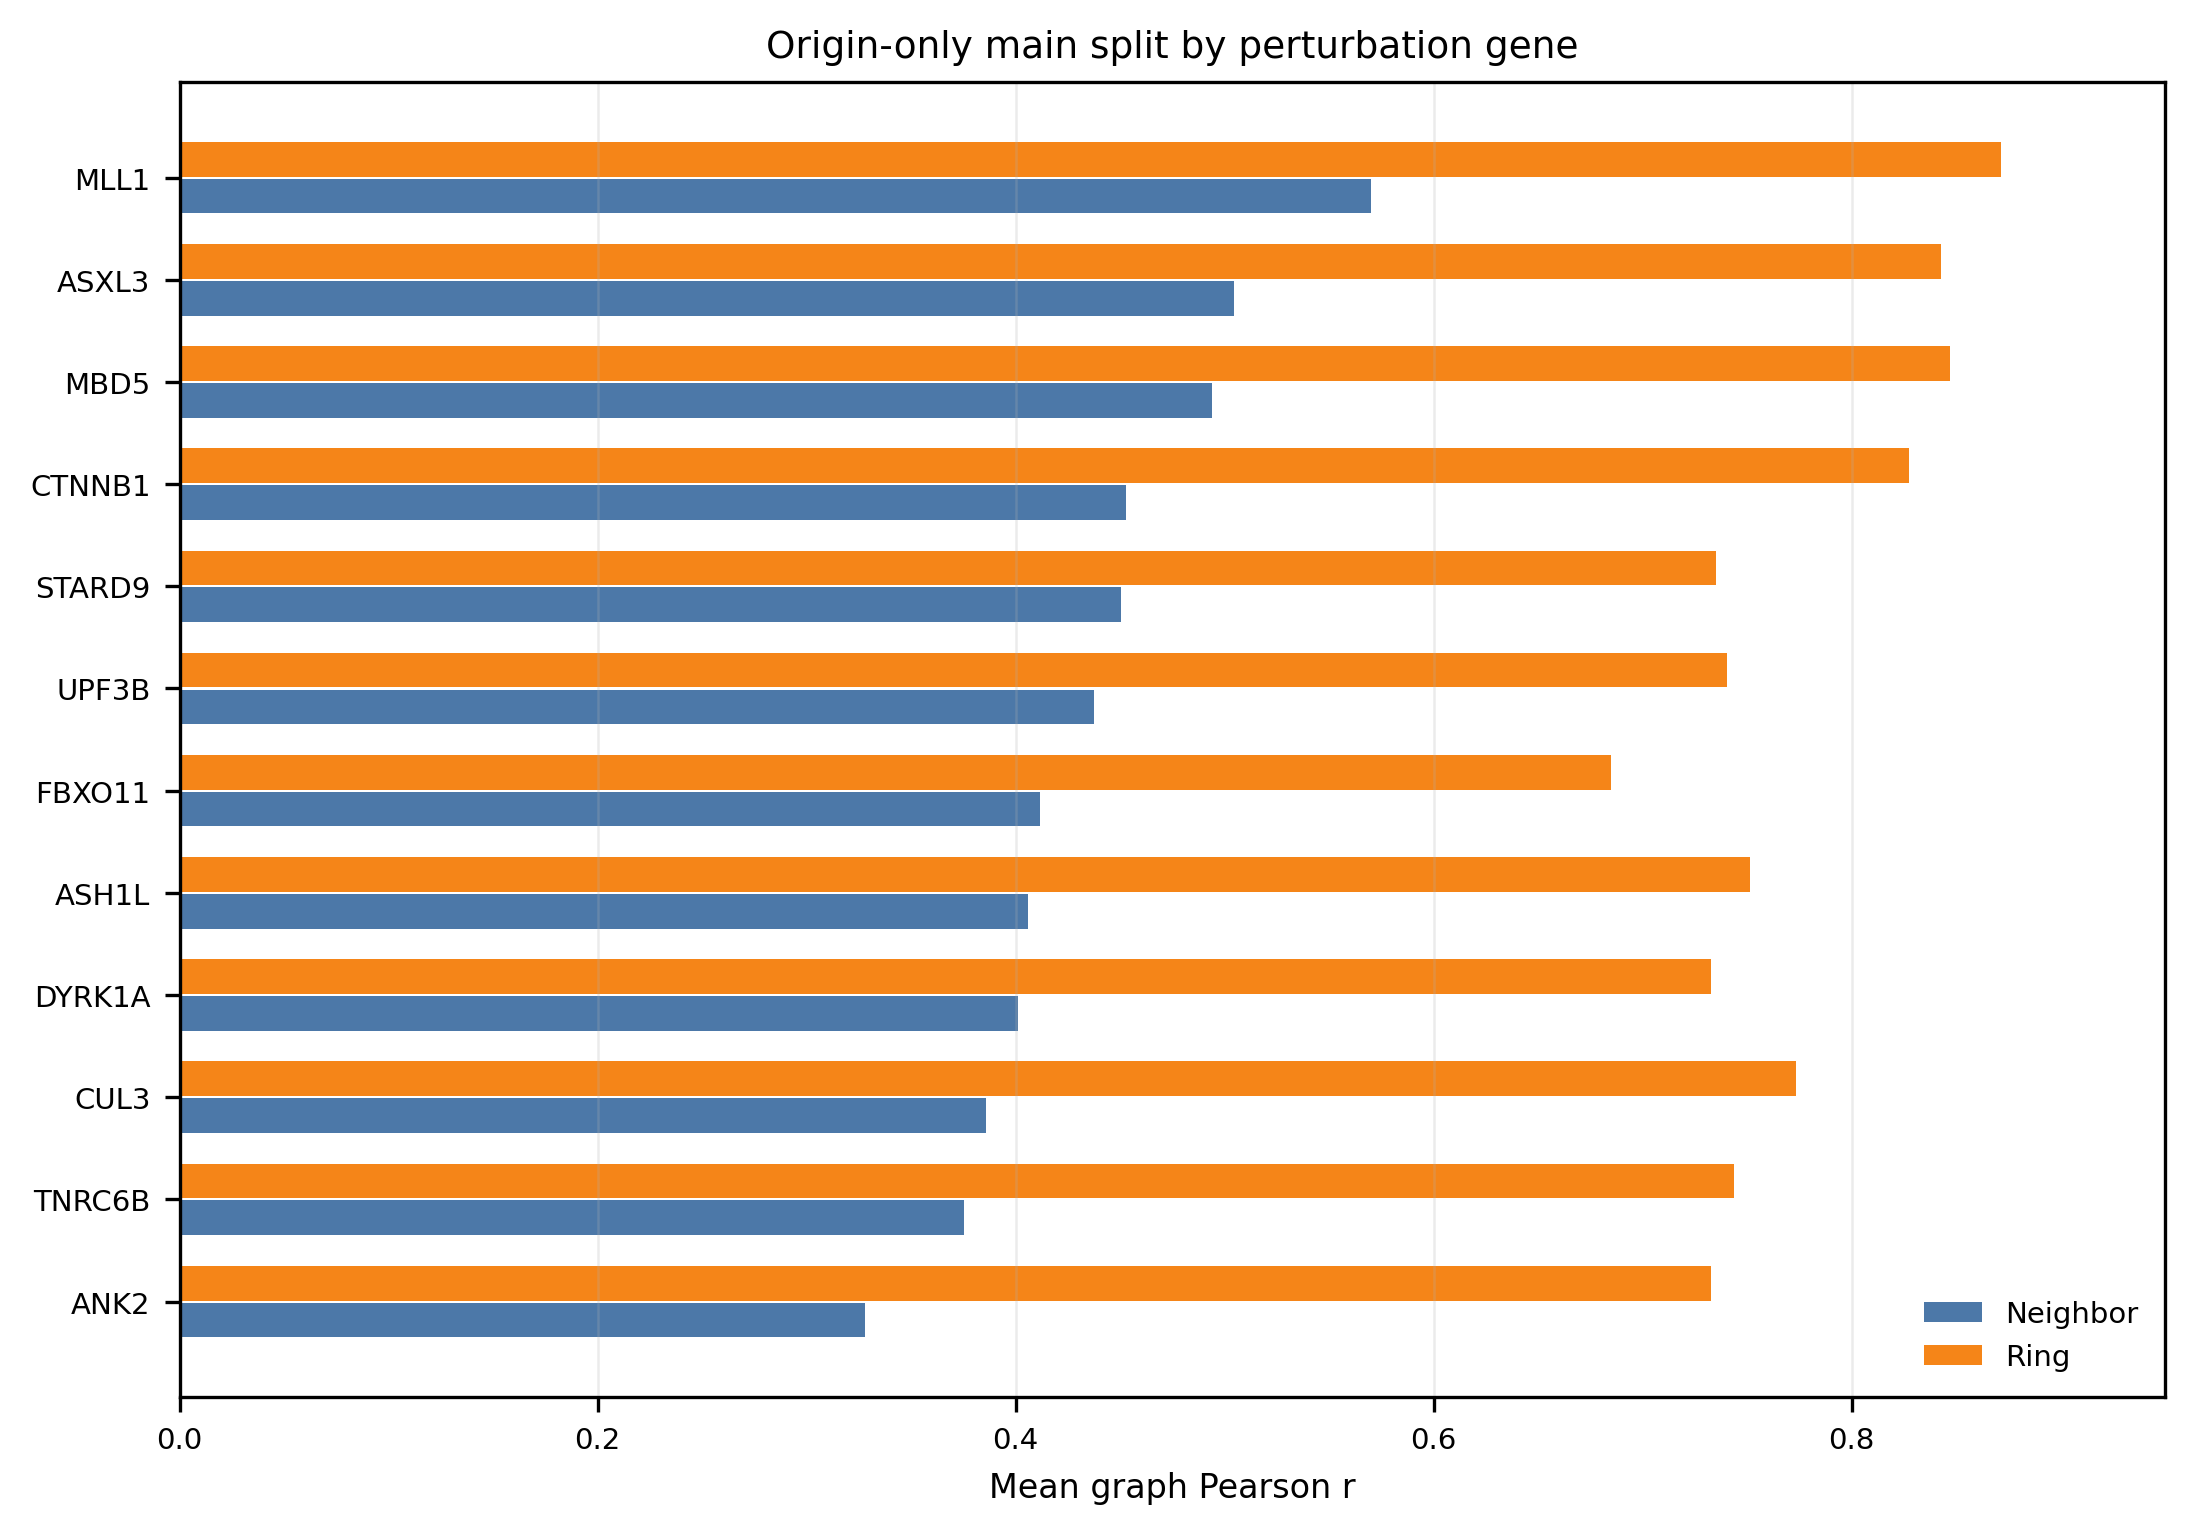
\includegraphics[width=0.5\linewidth]{synthetic_lr_gene_breakdown.png}
    \caption{\textbf{Main-split synthetic benchmark by perturbation gene.}
    Bars show mean graph Pearson $r$ for neighbor and ring-level recovery,
    ranked by perturbation gene. Ring-level recovery remains strong across perturbation
    genes, while neighbor recovery varies more across perturbation identities.}
    \label{fig:synthetic_lr_gene_breakdown}
\end{figure}

\begin{table}[t]
\centering
\small
\setlength{\tabcolsep}{4pt}
\renewcommand{\arraystretch}{1.08}
\caption{\textbf{Main model comparison on the controlled synthetic LR-propagation benchmark.}
Synthetic fine-tuning substantially improves neighbor and ring-level recovery
relative to niche-module-only prediction and direct transfer from the real-data pretrained model.}
\label{tab:synthetic_lr_main_models}
\begin{tabular}{lcccccc}
\toprule
Model & Neighbor & Centered & Ring & Center & $\Delta$Nei. & $\Delta$Ring \\
\midrule
Niche module only & 0.0033 & 0.0012 & 0.0062 & -0.0047 & 0.0000 & 0.0000 \\
Pretrained, $\alpha=0$ & 0.0663 & 0.0087 & 0.1281 & 0.5003 & 0.0631 & 0.1219 \\
Pretrained, $\alpha=0.75$ & 0.0692 & 0.0097 & 0.1320 & 0.5008 & 0.0659 & 0.1258 \\
Pretrained, $\alpha=1$ & 0.0699 & 0.0101 & 0.1327 & 0.5003 & 0.0666 & 0.1265 \\
Synthetic fine-tuned & \textbf{0.6193} & \textbf{0.3142} & \textbf{0.8148} & \textbf{0.9971} & \textbf{0.6160} & \textbf{0.8086} \\
\bottomrule
\end{tabular}
\end{table}

\begin{table*}[t]
\centering
\small
\setlength{\tabcolsep}{4pt}
\renewcommand{\arraystretch}{1.08}
\caption{\textbf{Cross-split robustness on the controlled synthetic LR benchmark.}
The synthetic-trained model generalizes across held-out interface geometry, held-out
strength, and held-out host-patch splits. The held-out perturbation split is more
challenging but remains non-trivial relative to the near-zero niche-module-only baseline.}
\label{tab:synthetic_lr_cross_split}
\begin{tabular}{lccccccccc}
\toprule
Split & Train & Val & Test & Niche nei. & Niche ring & Trained nei. & Centered & Trained ring & Gain nei. / ring \\
\midrule
Main stratified & 252 & 72 & 108 & 0.0033 & 0.0062 & 0.6193 & 0.3142 & 0.8148 & 0.6160 / 0.8086 \\
Held-out perturbation & 252 & 72 & 108 & 0.0037 & 0.0095 & 0.2743 & 0.1842 & 0.5503 & 0.2706 / 0.5408 \\
Held-out interface & 240 & 48 & 144 & 0.0038 & 0.0076 & 0.6070 & 0.3207 & 0.8056 & 0.6032 / 0.7981 \\
Held-out strength $2.0$ & 240 & 48 & 144 & 0.0040 & 0.0089 & 0.5201 & 0.2273 & 0.8068 & 0.5161 / 0.7979 \\
Held-out host patch & 252 & 72 & 108 & 0.0030 & 0.0056 & 0.5970 & 0.2269 & 0.8063 & 0.5940 / 0.8006 \\
\bottomrule
\end{tabular}
\end{table*}

\begin{table}[t]
\centering
\small
\setlength{\tabcolsep}{5pt}
\renewcommand{\arraystretch}{1.08}
\caption{\textbf{Simulator mismatch and null controls.}
The trained model transfers weakly to mismatched or null simulators, supporting the
interpretation that the main synthetic benchmark tests a specific LR-propagation
distribution rather than generic target leakage.}
\label{tab:synthetic_lr_mismatch_null}
\begin{tabular}{lcccc}
\toprule
Simulator & $n$ graphs & Trained nei. & Trained ring & Gain nei. / ring \\
\midrule
Direct distance & 360 & 0.0727 & 0.0994 & 0.0700 / 0.0948 \\
LIANA LR proxy & 360 & 0.0739 & 0.1022 & 0.0715 / 0.0989 \\
Random ligand--target & 360 & 0.2135 & 0.3144 & 0.2120 / 0.3141 \\
Shuffled direct effect & 360 & 0.0357 & 0.0359 & 0.0332 / 0.0312 \\
\bottomrule
\end{tabular}
\end{table}

\begin{table*}[t]
\centering
\small
\setlength{\tabcolsep}{4pt}
\renewcommand{\arraystretch}{1.08}
\caption{\textbf{Main-split breakdown by geometry, strength, direct-effect fraction, and radius scale.}
Niche-module-only predictions remain near zero across construction factors. Synthetic fine-tuning
recovers strong ring-level structure across all tested settings.}
\label{tab:synthetic_lr_factor_breakdown}
\begin{tabular}{llcccccc}
\toprule
Factor & Setting / model & $n$ & Neighbor & Nei. SEM & Centered & Ring & Ring SEM \\
\midrule
\multicolumn{8}{l}{\textit{Geometry strategy}} \\
Cluster, niche-only & -- & 36 & 0.0077 & 0.0014 & 0.0023 & 0.0158 & 0.0035 \\
Interface, niche-only & -- & 36 & 0.0044 & 0.0010 & 0.0009 & 0.0150 & 0.0035 \\
Random, niche-only & -- & 36 & 0.0063 & 0.0014 & 0.0016 & 0.0166 & 0.0030 \\
Cluster, trained & -- & 36 & 0.4608 & 0.0164 & 0.3755 & 0.8159 & 0.0098 \\
Interface, trained & -- & 36 & 0.4491 & 0.0148 & 0.3556 & 0.8011 & 0.0136 \\
Random, trained & -- & 36 & 0.3975 & 0.0174 & 0.2993 & 0.7069 & 0.0228 \\
\midrule
\multicolumn{8}{l}{\textit{Perturbation strength}} \\
0.75, niche-only & -- & 36 & 0.0068 & 0.0013 & 0.0015 & 0.0160 & 0.0029 \\
1.25, niche-only & -- & 36 & 0.0047 & 0.0012 & 0.0008 & 0.0147 & 0.0033 \\
2.00, niche-only & -- & 36 & 0.0069 & 0.0014 & 0.0025 & 0.0167 & 0.0037 \\
0.75, trained & -- & 36 & 0.4323 & 0.0153 & 0.3444 & 0.7538 & 0.0201 \\
1.25, trained & -- & 36 & 0.4391 & 0.0143 & 0.3439 & 0.7931 & 0.0118 \\
2.00, trained & -- & 36 & 0.4359 & 0.0204 & 0.3421 & 0.7769 & 0.0208 \\
\midrule
\multicolumn{8}{l}{\textit{Direct-effect fraction}} \\
0.05, niche-only & -- & 54 & 0.0064 & 0.0011 & 0.0016 & 0.0163 & 0.0025 \\
0.10, niche-only & -- & 54 & 0.0058 & 0.0010 & 0.0016 & 0.0153 & 0.0029 \\
0.05, trained & -- & 54 & 0.4309 & 0.0127 & 0.3464 & 0.7638 & 0.0139 \\
0.10, trained & -- & 54 & 0.4407 & 0.0146 & 0.3405 & 0.7854 & 0.0156 \\
\midrule
\multicolumn{8}{l}{\textit{Radius scale}} \\
0.50, niche-only & -- & 54 & 0.0059 & 0.0008 & 0.0017 & 0.0167 & 0.0024 \\
1.00, niche-only & -- & 54 & 0.0063 & 0.0012 & 0.0015 & 0.0149 & 0.0030 \\
0.50, trained & -- & 54 & 0.4470 & 0.0145 & 0.3915 & 0.7687 & 0.0158 \\
1.00, trained & -- & 54 & 0.4246 & 0.0127 & 0.2955 & 0.7806 & 0.0137 \\
\bottomrule
\end{tabular}
\end{table*}

\begin{table}[t]
\centering
\small
\setlength{\tabcolsep}{5pt}
\renewcommand{\arraystretch}{1.08}
\caption{\textbf{Synthetic benchmark by perturbation gene on the main split.}
Perturbation genes are ranked by neighbor Pearson.}
\label{tab:synthetic_lr_gene_breakdown}
\begin{tabular}{lcccc}
\toprule
Perturbation gene & $n$ graphs & Neighbor & Centered & Ring \\
\midrule
\textit{MLL1} & 11 & 0.5699 & 0.4459 & 0.8713 \\
\textit{ASXL3} & 7 & 0.5046 & 0.4149 & 0.8429 \\
\textit{MBD5} & 7 & 0.4938 & 0.4248 & 0.8471 \\
\textit{CTNNB1} & 9 & 0.4529 & 0.3684 & 0.8274 \\
\textit{STARD9} & 12 & 0.4503 & 0.3751 & 0.7349 \\
\textit{UPF3B} & 12 & 0.4373 & 0.3812 & 0.7404 \\
\textit{FBXO11} & 3 & 0.4117 & 0.3436 & 0.6850 \\
\textit{ASH1L} & 8 & 0.4061 & 0.3418 & 0.7513 \\
\textit{DYRK1A} & 13 & 0.4013 & 0.2635 & 0.7329 \\
\textit{CUL3} & 9 & 0.3857 & 0.3115 & 0.7737 \\
\textit{TNRC6B} & 7 & 0.3751 & 0.3115 & 0.7440 \\
\textit{ANK2} & 10 & 0.3279 & 0.1748 & 0.7328 \\
\bottomrule
\end{tabular}
\end{table}

\paragraph{Interpretation.}
The controlled synthetic benchmark supports three conclusions. First, niche-module-only
prediction remains near zero, so the synthetic response field is not recoverable from
tissue context alone. Second, synthetic fine-tuning generalizes well across held-out
graphs and construction factors, especially geometry, strength, direct-effect fraction, and
radius scale. Third, the held-out perturbation split is substantially harder than the
main stratified split, indicating that unseen perturbation identity remains the main
synthetic generalization bottleneck. We therefore use this benchmark as controlled
validation of direct-effect-conditioned propagation under known LR simulation rules, not as
a replacement for the real cell-resolved Spatial Perturb-Seq benchmark.

\subsection{Spot- and lesion-level external validation on Perturb-map / GSE193460}
\label{app:perturbmap_validation}

Perturb-map / GSE193460 provides a real spatial CRISPR validation setting with
spot- or lesion-level perturbation readouts. Because it does not provide matched
cell-resolved neighbor-response targets, we do not use it as an exact benchmark.
Instead, we aggregate \methodname{} predictions to spot-level and lesion-level gene
programs and compare them with observed perturbation-associated spatial signatures.

\begin{table}[t]
\centering
\small
\setlength{\tabcolsep}{4pt}
\renewcommand{\arraystretch}{1.08}
\caption{\textbf{Perturb-map / GSE193460 external validation.}
Spot-level Pearson correlations compare predicted and observed program scores.
Lesion-level Spearman correlations compare lesion-level ranking of perturbation-associated
programs.}
\label{tab:perturbmap_external}
\begin{tabular}{lcc}
\toprule
Readout & Spot Pearson $r$ & Lesion Spearman $\rho$ \\
\midrule
\textit{Ifngr2} top-25 program & 0.8528 & 0.5357 \\
\textit{Jak2} top-25 program & 0.7569 & 0.9286 \\
\textit{Tgfbr2} top-25 program & 0.7138 & 0.6071 \\
Curated TGF$\beta$--stroma program & 0.8076 & 0.7500 \\
IFN-response program & 0.6275 & -- \\
\bottomrule
\end{tabular}
\end{table}

\begin{table}[t]
\centering
\small
\setlength{\tabcolsep}{5pt}
\renewcommand{\arraystretch}{1.08}
\caption{\textbf{Top-$k$ sensitivity for Perturb-map spot-level validation.}
Top-50 equals top-25 because the common-gene mask does not add additional usable
genes beyond the top-25 set.}
\label{tab:perturbmap_topk}
\begin{tabular}{lccc}
\toprule
Signature & Top-10 & Top-25 & Top-50 \\
\midrule
\textit{Ifngr2} spot Pearson & 0.8252 & 0.8528 & 0.8528 \\
\textit{Jak2} spot Pearson & 0.7063 & 0.7569 & 0.7569 \\
\textit{Tgfbr2} spot Pearson & 0.6292 & 0.7138 & 0.7138 \\
\bottomrule
\end{tabular}
\end{table}

\begin{table}[t]
\centering
\small
\setlength{\tabcolsep}{5pt}
\renewcommand{\arraystretch}{1.08}
\caption{\textbf{Bootstrap confidence intervals and null controls for Perturb-map validation.}
All interpretable spot-level programs are significant against score-permutation nulls
($p=0.001$). The random gene-program null is stricter and supports selected readouts.}
\label{tab:perturbmap_null_ci}
\begin{tabular}{lccc}
\toprule
Readout & Observed score & 95\% bootstrap CI & Random program null $p$ \\
\midrule
\textit{Ifngr2} top-25 spot Pearson & 0.8528 & [0.8114, 0.8867] & 0.0150 \\
\textit{Jak2} top-25 spot Pearson & 0.7569 & [0.7019, 0.8014] & trend \\
\textit{Tgfbr2} top-25 spot Pearson & 0.7138 & [0.6647, 0.7545] & trend \\
Curated TGF$\beta$--stroma spot Pearson & 0.8076 & [0.7648, 0.8423] & 0.0040 \\
\textit{Jak2} lesion Spearman & 0.9286 & -- & 0.0490 \\
\bottomrule
\end{tabular}
\end{table}

\paragraph{Interpretation.}
Perturb-map provides a coarse external validation setting rather than a matched
cell-resolved propagation benchmark. The spot-level correlations are high and stable
under bootstrap resampling, and the top-$k$ sensitivity analysis shows that the
program-level agreement is not specific to a single top-$k$ threshold. Score-permutation
nulls are significant for all interpretable programs, while the stricter random
gene-program null supports the curated TGF$\beta$--stroma program, the \textit{Ifngr2}
top-25 spot program, and the \textit{Jak2} lesion-level ranking. These results support
cross-assay alignment of \methodname{} response fields under coarser Perturb-map
supervision, while preserving the primary role of Spatial Perturb-Seq as the exact
cell-resolved benchmark.

\subsection{Complete system-level baseline comparison}
\label{app:full_baseline_comparison}

\begin{table*}[t]
\centering
\caption{Complete system-level baseline comparison on the block-holdout Spatial Perturb-seq benchmark. Neighbor, neighbor-centered, high-confidence neighbor, and ring metrics are Pearson correlations; higher is better. MAE is lower better.}
\label{tab:app_full_baseline_comparison}
\scriptsize
\setlength{\tabcolsep}{3pt}
\renewcommand{\arraystretch}{1.12}
\begin{tabularx}{\textwidth}{@{}>{\raggedright\arraybackslash}p{0.11\textwidth}
>{\raggedright\arraybackslash}X
>{\raggedright\arraybackslash}p{0.16\textwidth}
ccccc@{}}
\toprule
Group & Method & Perturbation input & Neigh. & N-centered & High-conf. & Ring & MAE \\
\midrule
Trivial &
Zero-delta / no-change &
none &
0.00000 & 0.00000 & 0.00000 & 0.00000 & 0.45344 \\

Niche &
Niche module only &
none &
0.60963 & 0.64284 & 0.50900 & 0.40510 & 0.43926 \\

Statistical &
Training-set guide mean &
guide ID &
0.00923 & 0.00000 & 0.01080 & 0.02657 & 0.46429 \\

Statistical &
Guide $\times$ cell-type $\times$ ring mean &
guide ID, cell type, ring &
0.00714 & -0.00045 & 0.00825 & 0.01731 & 0.46752 \\

Retrieval &
Nearest matched training patch transfer &
matched patch &
0.00012 & -0.00104 & 0.00060 & 0.00960 & 0.61186 \\

Linear &
Elastic-net patch regression &
patch features &
0.56953 & 0.59375 & 0.56896 & 0.39101 & 0.42737 \\

Generic graph &
GAT / GraphSAGE patch model &
graph features &
0.54532 & 0.56623 & 0.54550 & 0.39668 & 0.46293 \\

Single-cell adapted &
Direct-effect predictor + distance diffusion &
predicted direct effect &
0.00616 & 0.00028 & 0.00664 & 0.01434 & 0.45912 \\

CCC adapted &
CCC-gated linear propagation &
fixed CCC &
-0.00191 & 0.00316 & -0.00224 & 0.00052 & 0.50968 \\

Ours &
Base direct-effect$\rightarrow$neighbor propagation &
measured direct effect &
0.68410 & 0.71701 & 0.68317 & 0.45204 & 0.40939 \\

\rowcolor{blue!7}
Ours &
\methodname{} final propagation blend &
measured direct effect + refinement &
0.68443 & 0.71566 & 0.68340 & 0.45722 & 0.40762 \\
\bottomrule
\end{tabularx}
\end{table*}

\paragraph{Baseline descriptions.}
The zero-delta baseline predicts no neighbor response. The niche-module-only patch model removes the direct-effect seed and direct-effect indicator, measuring how much local tissue context alone explains the target. Statistical baselines use training-set guide means or guide--cell-type--ring means. The retrieval baseline transfers neighbor deltas from the nearest matched training patch. The elastic-net row is the strongest shallow linear predictor among ridge and elastic-net variants. The generic graph baseline uses the same graph inputs as \methodname{} but removes niche-impact residualization, direct-effect-to-neighbor restriction, and ring feedback. The single-cell adapted baseline predicts a cell-autonomous direct effect and diffuses it by distance or ring kernels. The CCC-gated baseline uses COMMOT/Spacia-style communication scores as fixed edge weights with a shallow propagation head. The two \methodname{} rows show the base niche--propagation direct-effect-to-neighbor model and the final propagation blend with ST-conditioned ring refinement.

\subsection{Aggregate gene-space metrics}
\label{app:gene_space_metrics}

\begin{table*}[t]
\centering
\caption{Aggregate gene-delta metrics for the same real-data run reported in the main gene-centric evaluation.}
\label{tab:app_gene_delta_metrics}
\small
\setlength{\tabcolsep}{5pt}
\renewcommand{\arraystretch}{1.12}
\begin{tabular}{lccccccc}
\toprule
Aggregation & Pearson & Spearman & Cosine & $R^2$ & MAE & RMSE & Sign acc. \\
\midrule
Flat all node--gene pairs & 0.679 & 0.336 & 0.679 & 0.460 & 0.417 & 0.857 & 0.483 \\
Flat neighbor pairs & 0.670 & 0.336 & 0.669 & 0.448 & 0.419 & 0.860 & 0.489 \\
Per-cell mean, all nodes & 0.690 & --- & 0.687 & 0.446 & 0.417 & 0.839 & 0.483 \\
Per-cell mean, neighbor cells & 0.686 & --- & 0.683 & 0.440 & 0.419 & 0.843 & 0.489 \\
\bottomrule
\end{tabular}
\end{table*}

At the flat gene-space level, the same run reaches Pearson/Spearman/Cosine $0.679/0.336/0.679$ over all node--gene pairs and $0.670/0.336/0.669$ on neighbor pairs. Aggregating first over cells yields mean per-cell Pearson $0.690$ overall and $0.686$ on neighbor cells.

\subsection{Propagation-blend sensitivity and reference-ST diagnostics}
\label{app:blend_and_reference_diagnostics}

\begin{table}[t]
\centering
\caption{Propagation-blend sensitivity on the held-out local benchmark. $\alpha=0$ is the base propagation module, and $\alpha=1$ is the reference-ST ring-refinement module.}
\label{tab:app_blend_sweep}
\small
\setlength{\tabcolsep}{5pt}
\renewcommand{\arraystretch}{1.10}
\begin{tabular}{cccccc}
\toprule
$\alpha$ & Neighbor & Neighbor-centered & Ring & Neighbor MAE & Score \\
\midrule
0.00 & 0.68410 & 0.71701 & 0.45204 & 0.40939 & 1.92869 \\
0.50 & 0.68467 & 0.71620 & 0.45667 & 0.40761 & 1.93692 \\
0.60 & 0.68453 & 0.71585 & 0.45708 & 0.40759 & 1.93733 \\
0.65 & 0.68443 & 0.71566 & 0.45722 & 0.40762 & \textbf{1.93737} \\
0.70 & 0.68430 & 0.71545 & 0.45731 & 0.40769 & 1.93730 \\
1.00 & 0.68309 & 0.71384 & 0.45681 & 0.40865 & 1.93438 \\
\bottomrule
\end{tabular}
\end{table}

The selected blend $\alpha=0.65$ gives the highest composite score in this sweep. The base propagation module is slightly stronger in neighbor-centered Pearson, while the reference-ST refinement improves ring structure.

\begin{table}[t]
\centering
\caption{Held-out diagnostics for the reference-ST microenvironment encoder. These metrics evaluate self-supervised pretraining objectives, not perturbation-response accuracy.}
\label{tab:app_organ_prior}
\small
\setlength{\tabcolsep}{8pt}
\renewcommand{\arraystretch}{1.12}
\begin{tabular}{lc}
\toprule
Diagnostic & Value \\
\midrule
Masked node-program loss & 1.13407 \\
Neighborhood-program loss & 0.45550 \\
Patch cell-type histogram loss & 0.01061 \\
Edge-prior loss & $3.8\times10^{-5}$ \\
Edge-prior correlation & 0.99439 \\
\bottomrule
\end{tabular}
\end{table}

The frozen reference encoder is trained only on unperturbed reference ST. These diagnostics verify that it learns stable microenvironment and edge-plausibility structure, but they should not be interpreted as perturbation-response accuracy.

\subsection{Development ablations}
\label{app:development_ablations}

The following tables retain the original development evidence but replace internal run names with descriptive labels. The early structural ablations show that explicit direct-effect-to-neighbor propagation is more effective than generic patch regression or purely semantic pairwise prediction. The recipe ablations show that longer optimization, three-control consensus targets, and post-state supervision improve earlier baselines, while strict same-type pseudo-pre targets are too noisy for the current local benchmark.

\begin{table*}[t]
\centering
\caption{Broad module and structural ablations from development runs, rewritten with descriptive labels.}
\label{tab:app_ablation_modules}
\small
\setlength{\tabcolsep}{8pt}
\renewcommand{\arraystretch}{1.14}
\begin{tabular}{@{}p{0.50\linewidth}ccc@{}}
\toprule
Variant & \makecell[c]{Direct-effect-cell\\Pearson} & \makecell[c]{Neighbor\\Pearson} & \makecell[c]{Ring\\Pearson} \\
\midrule
\textbf{Full structured propagation}, spatial block holdout & 0.959 & 0.670 & 0.421 \\
Niche-module-only region-patch baseline, spatial block holdout & 1.000 & 0.610 & 0.405 \\
\textbf{Structured propagation}, earlier coordinate split & 0.963 & 0.643 & 0.375 \\
Structured propagation without post-state loss, earlier coordinate split & 0.963 & 0.640 & 0.373 \\
Semantic propagation module, earlier coordinate split & 0.983 & 0.607 & 0.426 \\
Direct-effect-indicator-only baseline, earlier coordinate split & 0.188 & 0.486 & 0.342 \\
Pair-only semantic-difference model, earlier coordinate split & 0.984 & 0.362 & 0.210 \\
\bottomrule
\end{tabular}
\end{table*}

\begin{table*}[t]
\centering
\caption{Training, target-construction, and split ablations from development runs, rewritten with descriptive labels. The last two rows are robustness or task-definition tests rather than standard leave-one-module-out ablations.}
\label{tab:app_ablation_recipe}
\small
\setlength{\tabcolsep}{8pt}
\renewcommand{\arraystretch}{1.14}
\begin{tabular}{@{}p{0.50\linewidth}p{0.43\linewidth}@{}}
\toprule
Recipe change & Key metrics \\
\midrule
Single-control target baseline: 10 $\rightarrow$ 30 epochs & neighbor $0.364\rightarrow0.509$; ring $0.236\rightarrow0.291$ \\
Single-control target $\rightarrow$ three-control consensus target, same 10-epoch baseline setting & neighbor $0.364\rightarrow0.425$; ring $0.236\rightarrow0.279$ \\
Three-control consensus target: 10 $\rightarrow$ 30 epochs & neighbor $0.425\rightarrow0.577$; ring $0.279\rightarrow0.355$ \\
Add post-state supervision to the region-patch baseline & neighbor $0.425\rightarrow0.536$; ring $0.279\rightarrow0.361$ \\
Coordinate-based split $\rightarrow$ spatial block holdout, strongest propagation model & neighbor $0.643\rightarrow0.670$; ring $0.375\rightarrow0.421$ \\
Matched-control target $\rightarrow$ strict same-cell-type aligned pseudo-pre target, stress test & full model: neighbor $0.0028$; ring $0.0000$ \\
\bottomrule
\end{tabular}
\end{table*}

\subsection{Detailed structural and design-refinement ablations}
\label{app:structural_design_refinement}

\begin{table*}[t]
\centering
\caption{Core structural ablations on the held-out local benchmark. Deltas are relative to the final propagation blend. The main paper reports the compact diagnostic summary; this table preserves the full structural-ablation values.}
\label{tab:app_core_structural_ablations}
\small
\setlength{\tabcolsep}{5pt}
\renewcommand{\arraystretch}{1.12}
\begin{tabularx}{\textwidth}{@{}>{\raggedright\arraybackslash}Xccccc@{}}
\toprule
Variant & Neighbor & Ring & MAE & $\Delta$Neighbor & $\Delta$Ring \\
\midrule
\rowcolor{cyan!10}
\methodname{} final propagation blend &
0.68443 & 0.45722 & 0.40762 & --- & --- \\

No niche-impact residualization &
0.16451 & 0.15320 & 0.69832 & $-0.51992$ & $-0.30402$ \\

No edge attributes &
0.60591 & 0.41819 & 0.43651 & $-0.07852$ & $-0.03903$ \\

No direct-effect input &
0.61405 & 0.44062 & 0.42917 & $-0.07038$ & $-0.01660$ \\
\bottomrule
\end{tabularx}
\end{table*}

\paragraph{Interpretation of structural ablations.}
The final propagation blend combines a shared niche-impact baseline with directed direct-effect-to-neighbor propagation and ring-aware refinement. Removing niche-impact residualization produces the largest collapse, indicating that directly predicting the response fails to separate background tissue variation from perturbation-conditioned propagation. Removing edge attributes reduces both neighbor and ring performance, showing that spatial geometry, cell-type-pair information, and communication-compatibility features improve propagation structure. Removing the direct-effect input also degrades neighbor prediction, especially beyond niche-module-only correlation, confirming that the propagation module benefits from a meaningful direct-effect signal.

\begin{table*}[t]
\centering
\caption{Design-refinement ablations. Deltas are reported relative to the stated reference model within each ablation family. Positive deltas mean the ablated comparison is better; negative deltas mean it is worse.}
\label{tab:app_design_refinement_ablations}
\small
\setlength{\tabcolsep}{4pt}
\renewcommand{\arraystretch}{1.12}
\begin{tabularx}{\textwidth}{@{}>{\raggedright\arraybackslash}p{0.22\textwidth}
>{\raggedright\arraybackslash}X
rrr@{}}
\toprule
Design question & Ablated comparison & $\Delta$Score & $\Delta$Neighbor & $\Delta$Ring \\
\midrule

Directed propagation &
Niche-module-only patch model $\rightarrow$ base direct-effect$\rightarrow$neighbor propagation &
--- & $+0.07447$ & $+0.04694$ \\

Ring-aware spatial refinement &
Base propagation module relative to reference-ST ring refinement &
$-0.00569$ & $+0.00101$ & $-0.00477$ \\

Reference niche integration &
Reference-niche adapter without response feedback &
$-0.00180$ & $+0.00014$ & $-0.00125$ \\

Reference prior placement &
Using the reference edge-prior signal directly &
$-0.00400$ & $-0.00057$ & $-0.00191$ \\

Feedback structure &
Plain second-pass refinement without ring-aware scaling &
$-0.00081$ & $+0.00022$ & $-0.00071$ \\

Reference-prior necessity &
Ring refinement without the reference-prior adapter &
$-0.00231$ & $+0.00106$ & $-0.00271$ \\

Neighbor-focused loss &
Including direct-effect-cell reconstruction in the propagation loss &
$-0.06372$ & $-0.01307$ & $-0.02665$ \\

Ring supervision &
Removing ring loss from the current module &
$-0.00150$ & $+0.00021$ & $-0.00113$ \\

\bottomrule
\end{tabularx}
\end{table*}

\paragraph{Interpretation of design-refinement ablations.}
The design-refinement ablations support the final architecture choices. Explicit direct-effect-to-neighbor propagation substantially improves neighbor prediction over the niche-module-only patch model. The base propagation module is slightly stronger in raw neighbor correlation than the reference-ST ring-refinement module, but weaker at ring-level spatial structure. Frozen reference context helps most when used inside ring-aware response refinement; using the reference edge-prior signal directly is weaker than injecting reference-ST information through node- and patch-level niche embeddings. A plain second pass is useful, but ring-aware response tokens and ring-specific scales give a better spatial tradeoff. Removing the reference-prior adapter slightly improves raw neighbor correlation but hurts ring propagation and the overall score. Including direct-effect-cell reconstruction in the propagation loss substantially hurts neighbor propagation, indicating that the easier direct signal can dominate training. Removing ring loss gives only a negligible raw-neighbor gain while reducing ring-level propagation structure.

\begin{table*}[t]
\centering
\caption{De novo IFN-$\gamma$ mouse-brain case-study readouts. This table supports a hypothesis-generating analysis, not a matched-ground-truth validation.}
\label{tab:app_ifng_case_readouts}
\footnotesize
\setlength{\tabcolsep}{4pt}
\renewcommand{\arraystretch}{1.16}
\begin{tabular}{@{}p{0.18\linewidth}p{0.40\linewidth}p{0.37\linewidth}@{}}
\toprule
Readout & Observation & Interpretation \\
\midrule
Top-pathway target composition &
Microglia: 11.91\% among top-pathway 5\% targets versus 7.98\% background; 1.49$\times$ enrichment. Endothelial: 7.81\% versus 7.22\%; 1.08$\times$ enrichment. Pericyte: 5.81\% versus 5.49\%; 1.06$\times$ enrichment. &
IFN-$\gamma$ susceptibility concentrates in immune/glial-associated niches and also involves vascular-associated microenvironments. \\

Canonical IFN/MHC-I genes &
Target-cell response: \textit{B2m} $+1.91$, \textit{H2-D1} $+1.57$, \textit{Ifitm3} $+1.72$. &
The de novo pipeline recovers a coherent IFN-$\gamma$/antigen-presentation-like program rather than arbitrary high-response genes. \\

Suppressed programs &
Target-cell response: \textit{Col1a2} $-1.31$, \textit{Vcan} $-1.28$, \textit{Flt1} $-1.82$. &
The predicted response includes suppression of selected ECM, structural, or vascular-like programs, not only inflammatory activation. \\

Spatial field coverage &
2,048 top-5\% targets; 64NN patch union covers 38,922/40,944 cells in the bottom-right region, or 95.06\%. &
The perturbation forms an extended spatial response field; target cells are strongest, but neighboring cells also show visible response. \\

Context-dependent gradients &
Patch-level $x$ coordinate is negatively associated with \textit{B2m} $(r=-0.290,\ p=4.2\times10^{-41})$ and \textit{Irf8} $(r=-0.296,\ p=8.8\times10^{-43})$, and positively associated with \textit{Col1a2} $(r=+0.307,\ p=5.7\times10^{-46})$ and \textit{Flt1} $(r=+0.417,\ p=7.4\times10^{-87})$. &
The same perturbation does not produce a uniform tissue-wide shift; local spatial context modulates response direction and strength. \\

Representative local patches &
Six representative patches: P1 $(x=14{,}955, y=8{,}981)$, P2 $(18{,}877, 11{,}976)$, P3 $(15{,}281, 12{,}090)$, P4 $(14{,}662, 15{,}755)$, P5 $(19{,}830, 17{,}042)$, and P6 $(16{,}754, 18{,}181)$. These patches show positive \textit{B2m}/\textit{Ifitm3} and negative \textit{Col1a2}/\textit{Vcan} patch-average responses. &
Local examples connect whole-map response gradients to neighborhood-scale propagation behavior. \\

Reference-prior deployment context &
The de novo query uses the frozen reference microenvironment prior during whole-brain deployment; no matched IFN-$\gamma$ labels or paired prior ablation are used for this table. &
The reference prior is framed as tissue contextualization for deployment, not as experimental validation of IFN-$\gamma$ biology or as the main source of raw benchmark Pearson improvement. \\
\bottomrule
\end{tabular}
\end{table*}

\subsection{Extended de novo IFN-\texorpdfstring{$\gamma$}{gamma} case-study interpretation}
\label{app:ifng_extended_interpretation}

\paragraph{External IFN-\texorpdfstring{$\gamma$}{gamma} direct-effect seed.}
The de novo IFN-$\gamma$ seed is generated from an external cytokine perturbation source rather than from the target ST slide. We train/fine-tune CPA on PerturbSapiens cytokine data with treatment status, cell type, and tissue/broad class as covariates. Treatment status distinguishes PBS/control and IFN-$\gamma$. For each Sample2/pre4 spatial cell, CPA is queried twice with the same cell and tissue covariates: once under the IFN-$\gamma$ condition and once under the PBS/control condition. The direct-effect seed is
\[
d_i^{\mathrm{IFN}\gamma}
=
\widehat{x}_{i}^{\mathrm{IFN}\gamma}
-
\widehat{x}_{i}^{\mathrm{PBS}} .
\]
The resulting per-cell direct delta is mapped to the benchmark gene set and used only as the direct-effect input for \methodname{} propagation. No paired IFN-$\gamma$ spatial perturbation label from the Sample2/pre4 tissue block is used during this inference.

\begin{table}[t]
\centering
\footnotesize
\setlength{\tabcolsep}{5pt}
\renewcommand{\arraystretch}{1.05}
\caption{Direct-effect seed construction for the de novo IFN-$\gamma$ mouse-brain case study.}
\label{tab:app_ifng_direct_effect_seed}
\begin{tabularx}{\linewidth}{lX}
\toprule
\textbf{Component} & \textbf{Specification} \\
\midrule
External perturbation source & PerturbSapiens cytokine data \\
Single-cell response model & CPA trained/fine-tuned on cytokine perturbation responses \\
Covariates & Treatment status, cell type, and tissue/broad class \\
Treatment contrast & IFN-$\gamma$ state minus PBS/control state \\
Spatial target cells & Sample2/pre4 mouse-brain spatial cells \\
Direct-effect seed & Per-cell delta $d_i^{\mathrm{IFN}\gamma}=\widehat{x}_{i}^{\mathrm{IFN}\gamma}-\widehat{x}_{i}^{\mathrm{PBS}}$ \\
Use in \methodname{} & Direct-effect input for spatial propagation; no paired IFN-$\gamma$ spatial labels are used \\
\bottomrule
\end{tabularx}
\end{table}

\paragraph{Spatial heterogeneity.}
The predicted response is not dominated by a single global offset. The whole-tissue maps identify regions with strong IFN-associated activation, while the local patch panels show that the signal extends into neighboring cells. Different genes show different response signs, and the same perturbation query produces region-dependent response magnitudes across selected patches.

\paragraph{Cell-state enrichment.}
The high-response regions are enriched for immune and glial-associated tissue context. Among top-pathway 5\% target cells, microglia account for 11.91\% of targets compared with a 7.98\% background frequency, corresponding to a 1.49$\times$ enrichment. Endothelial and pericyte states are mildly enriched as well, at 7.81\% versus 7.22\% and 5.81\% versus 5.49\%, respectively. This suggests that the de novo response field is concentrated in immune-, vascular-, and glial-associated niches rather than assigned uniformly across the tissue.

\paragraph{Gene-program response.}
At the gene-program level, the model predicts a coherent IFN-$\gamma$/MHC-I-like response. Target-cell deltas are positive for canonical interferon and antigen-presentation genes, including \textit{B2m} $(+1.91)$, \textit{H2-D1} $(+1.57)$, and \textit{Ifitm3} $(+1.72)$. In parallel, selected structural or vascular-associated programs are suppressed, including \textit{Col1a2} $(-1.31)$, \textit{Vcan} $(-1.28)$, and \textit{Flt1} $(-1.82)$. The selected local patches recapitulate this pattern at neighborhood scale: patch-averaged deltas are consistently positive for \textit{B2m} and \textit{Ifitm3}, and consistently negative for \textit{Col1a2} and \textit{Vcan}. Across the six displayed patches, \textit{B2m} averages range from $+0.69$ to $+0.96$, \textit{Ifitm3} from $+0.24$ to $+0.33$, while \textit{Col1a2} and \textit{Vcan} remain negative.

\paragraph{Extended spatial field.}
The predicted response forms an extended spatial field. The 64-nearest-neighbor union around 2,048 top-5\% targets covers 38,922 of 40,944 cells in the analyzed bottom-right region, or 95.06\%. Thus, the deployment output should be interpreted as a tissue-level response field rather than a set of isolated target-cell predictions. Consistent with this interpretation, patch-level spatial gradients show that the $x$ coordinate is negatively associated with \textit{B2m} response $(r=-0.290,\ p=4.2\times10^{-41})$ and \textit{Irf8} response $(r=-0.296,\ p=8.8\times10^{-43})$, and positively associated with \textit{Col1a2} response $(r=+0.307,\ p=5.7\times10^{-46})$ and \textit{Flt1} response $(r=+0.417,\ p=7.4\times10^{-87})$.

\paragraph{Role of the reference microenvironment prior.}
In the paired benchmark, the reference microenvironment module is a secondary ring-level refinement rather than the main source of Neighbor Pearson improvement. In de novo whole-brain deployment, however, the frozen reference prior provides tissue-contextual information that helps map the same perturbation query onto susceptible microenvironments and generate a heterogeneous response field. The IFN-$\gamma$ analysis should therefore be read as a biologically grounded deployment example, not as experimental validation of IFN-$\gamma$ biology.

\subsection{Extended discussion}
\label{app:extended_discussion}

\paragraph{Controlled propagation versus de novo perturbation prediction.}
\methodname{} separates two problems that are often conflated in spatial perturbation modeling. The benchmark evaluates propagation conditioned on a direct-effect profile, while de novo use additionally requires a model that maps perturbation identity to that profile. This separation avoids attributing errors in direct-effect prediction to the spatial propagation module, and it makes the neighbor-response task directly measurable with Spatial Perturb-Seq supervision.

\paragraph{Role of niche-impact residualization.}
Matched-control construction, local anatomy, and cell-type composition explain a substantial fraction of the observed neighbor response field. A model that predicts the full delta directly can therefore obtain high flat neighbor correlation by fitting tissue context rather than perturbation-conditioned propagation. Niche-impact residualization reduces this shortcut: the niche module accounts for background tissue variation, and the propagation module is forced to explain direct-effect-driven response beyond that baseline.

\paragraph{Why ring lift matters.}
Flat Neighbor Pearson is not a sufficient diagnostic of perturbation conditioning, because several direct-effect perturbation controls retain high Neighbor Pearson through the niche module. Ring-level lift is more sensitive to whether perturbation information changes the radial organization of neighbor response. The measured direct-effect model produces the largest ring lift over niche-module-only prediction, whereas shuffled or noisy controls largely collapse back toward the niche-impact baseline.

\paragraph{Use of ST-mined microenvironment priors.}
The reference-ST encoder is pretrained from unperturbed spatial transcriptomics and frozen before perturbation training. It is used to provide tissue-contextual information, including local niche structure and communication plausibility, but it does not provide perturbation-response labels. In the paired benchmark, this prior mainly contributes a modest ring-level refinement. In de novo whole-brain inference, it helps contextualize which microenvironments are susceptible to the same perturbation query.

\paragraph{Interpretation of the IFN-$\gamma$ case study.}
The IFN-$\gamma$ analysis should be read as a hypothesis-generating deployment demonstration rather than a matched experimental validation. It shows that a perturbation-identity-derived direct-effect profile can produce spatially heterogeneous response fields, recover canonical IFN/MHC-I-like genes, suppress selected structural or vascular-like programs, and generate local response gradients. These outputs illustrate the intended deployment interface, but their biological claims require direct experimental validation.

\subsection{Whole-block visualization wrapper}
\label{app:whole_block_wrapper}

The quantitative benchmark is local and matched-control based. For whole-block visualization, we keep the same trained local model but change only the inference layout. Predictions are first generated in matched-control patch coordinates, then softly projected onto the post-perturbation layout using same-cell-type, relative-position, and expression-similarity correspondence. Patch predictions are merged by post anchors rather than control donor rows, preventing control-patch deduplication from collapsing spatial coverage. This wrapper is used for visualization and external-study deployment; it is not mixed with the local paired-patch metrics.


\subsection{Experiment compute resources}
\label{app:compute_resources}

All experiments were run on a Linux workstation with NVIDIA RTX A6000 GPUs. Each GPU has 48 GB memory. The reference machine had 8 GPUs available, but each released training or evaluation command uses a single GPU by default through \texttt{--device cuda}. The machine had 64 logical CPU threads and 1 TB system RAM. CPU and storage throughput mainly affect raw-data preprocessing and graph construction; model training uses compact fixed-size graph patches.

Unless otherwise stated, \methodname{} experiments use 64-cell graph patches. The released scripts expose all compute-relevant settings, including batch size, epoch count, learning rate, device flag, split setting, and random seed.

\paragraph{Main \methodname{} experiment.}
Dataset construction uses patch size 64, a spatial-block split, training blocks \texttt{top\_right} and \texttt{bottom\_left}, test block \texttt{bottom\_right}, consensus target aggregation, and 5 matched controls per anchor. The niche module uses hidden dimension 256, 3 encoder layers, 3 propagation layers, batch size 16, 30 epochs, and learning rate $3\times10^{-4}$. The residual direct-effect-to-neighbor model uses hidden dimension 256, 3 propagation layers, batch size 16, 10 epochs, and learning rate $3\times10^{-4}$.

The reference-ST niche prior model uses patch size 64, edge $k=8$, local CCC top-$k=5$, 4096/512/512 train/validation/test samples, hidden dimension 128, batch size 32, 20 epochs, and learning rate $10^{-3}$. The organ-ring refinement uses batch size 16: the organ-adapter stage runs for 10 epochs at $5\times10^{-4}$, the response-refine stage for 6 epochs at $2\times10^{-4}$, the ring-refine stage for 6 epochs at $10^{-4}$, and the final organ-ring stage for 6 epochs at $7.5\times10^{-5}$. Best-model evaluation uses batch size 16 and sweeps $\alpha\in\{0.0,0.25,0.5,0.55,0.6,0.65,0.7,0.75,1.0\}$.

\paragraph{Ablations and baselines.}
OrganRingBlend ablations use the same residual graph model with hidden dimension 256, 3 propagation layers, batch size 16, and 6--10 epochs depending on the ablation. Seed and shortcut controls use batch size 16 and random seed 0. The shallow MLP baseline uses hidden dimension 512, batch size 8192, 20 epochs, and learning rate $10^{-3}$. Source/radial and summary baselines are CPU-light evaluation jobs.

\paragraph{Validation experiments.}
For Perturb-map / GSE193460, pseudo-ground-truth construction uses 64-cell patches and CPU preprocessing. Leave-one-out fine-tuning uses batch size 4, 80 epochs, learning rate $3\times10^{-4}$, and weight decay $10^{-4}$. Masked external evaluation and program validation use batch size 4. Robustness analysis uses 1000 null trials.

For GSE157977 synthetic ligand--receptor validation, direct-profile construction and gene-space projection are CPU preprocessing steps. Synthetic graph construction uses random seed 0. Direct-effect ablation evaluation uses batch size 16 and GPU evaluation.

For Perturb-FISH validation, graph construction uses 64-cell patches, at most 25 centers per perturbation, at least 5 positive cells, and random seed 11. The native ridge effect model uses $\alpha\in\{0.01,0.1,1,10,100,1000\}$ and 1000 null trials. The native \methodname{} graph model uses hidden dimension 256, 3 propagation layers, batch size 16, 30 epochs, learning rate $3\times10^{-4}$, weight decay $10^{-4}$, and patience 8.

\paragraph{Optional foundation-adapter experiments.}
CellPLM embedding construction uses batch size 512 and \texttt{cuda:0}. scGPT embedding construction uses batch size 32 and \texttt{cuda:0}. Frozen expression+niche adapters use CPU feature construction followed by the same \methodname{} residual training settings described above.

Exact wall-clock time depends on GPU model, CPU memory, and storage throughput. The released code package specifies the hardware class and all per-experiment compute settings needed to reproduce the reported experiments.




\end{document}